
\chapter{A binomiális együtthatók és a Pascal-háromszög}\label{chap:Pascal}
\begin{description}
	{\large \item [{Szerző:}] Seress Brigitta-Alexandra (Korszerű módszerek a matematikatanításban, Didaktikai mesteri -- Matematika, 
	II. év)}
\end{description}
\vspace{0.5cm}


\textbf{1. Történelmi áttekintés}

\vspace{0.3cm}

\textbf{\textit{I. Binomiális tétel és Pascal-háromszög elődjei}}

A \textcolor{ccqqqq}{binomiális együtthatók háromszögbe rendezése},
valamint a {\color{ccqqqq}{binomiális tétel kisebb pozitív egész
kitevőkre}} való alkalmazása már a következő matematikusok munkásságaiban
is fellelhető: 
\begin{itemize}
\item \textbf{Al-Karaji} (10. századi arab matematikus) 
\item \textbf{Omar Khayyam} (11. századi arab matematikus) 
\item \textbf{Yang Hui} (13. századi kínai matematikus) 
\item Pascal-háromszöget így ismerik: 
\begin{itemize}
\item Iránban: \textbf{"Khajjám-háromszög"} 
\item Kínában: \textbf{„Yang Hui-háromszög”} (lásd \ref{7sb1}. ábra). 
\end{itemize}
\end{itemize}
\begin{figure}[h]
\centering \includegraphics[width=5cm,height=7cm]{\string"content/Seres_Brigitta_Alexandra/1\string".JPG}
\caption{Yang Hui-háromszög kínai ábrázolása}
\label{7sb1} 
\end{figure}

\vspace{0.3cm}

\textbf{\textit{II. Pascal-háromszög Európában}} 
\begin{itemize}
\item[{\Large\textbf{1527:}}] \textbf{Petrus Apianus} német reneszánsz tudós a \textcolor{ccqqqq}{nyugati
világban elsőként} (a névadó Blaise Pascal előtt) foglalkozott a
"Pascal-háromszög" egy változatával. 
\item[{\Large\textbf{1553:}}] \textbf{Michael Stifel} német matematikus közölte a „Pascal-háromszöget",
\textcolor{ccqqqq}{bevezette a "binomiális együttható"} kifejezést. 
\item[{\Large\textbf{1556:}}] \textbf{Nicolo Tartaglia} olasz matematikus "Pascal-háromszöggel"
kapcsolatos írást közöl \textit{"General Trattato di Numeri et Misure,
Part II"} című könyvében. \textbf{Olaszországban} a mai napig \textcolor{ccqqqq}{„Tartaglia-háromszögként”}
hivatkoznak a Pascal-háromszögre. 
\item[{\Large\textbf{1665:}}] \textbf{Blaise Pascal} francia polihisztor a \textit{"Traité du
triangle arithmétique"} című értekezésében \textcolor{ccqqqq}{összegyűjtötte
a háromszögre vonatkozó akkor ismert adatokat és valószínűségszámítási
feladatok megoldására használta}. 
\item A háromszöget utóbb \textbf{Pierre Raymond de Montmort} (1708) és
\textbf{Abraham de Moivre} (1730) nevezte el Pascalról. 
\end{itemize}
\vspace{0.3cm}

\textbf{\textit{III. Binomiális tétel Európában}}
\begin{itemize}
\item \textbf{James Gregory} (17. századi skót matematikus): 
\begin{itemize}
\item \textbf{1670}: teljesen önállóan \textcolor{ccqqqq}{általánosította
a binomiális tételt törtkitevőkre} is (ugyan megvolt már Newton hasonló
eredménye, de "csak" íróasztalának fiókjában), 
\item Newton egyetemista korában Gregory Cambridge-ben tanított, így nincs
kizárva, hogy tanította Newtont. 
\end{itemize}
\item \textbf{Isaac Newton} (17. századi angol matematikus): 
\begin{itemize}
\item \textcolor{ccqqqq}{első matematikai felfedezései} közé tartozik
a \textcolor{ccqqqq}{\textbf{binomiális tétel általánosítása }\textbf{\textit{valós}}\textbf{
kitevőkre (1665)}}, Gregorytól függetlenül (aki közlésben megelőzte), 
\item \textbf{eredményét 1676-ban} írta meg két levélben Henry Oldenburgnak, 
\item Newton leveléből kitűnik, hogy a binomiális tétel általánosítása egy
\textit{szűk függvényosztály sorbafejtésének az érdekében történt,
hogy azután lehetővé váljék a tagonkénti integrálás}, 
\item Newton beleegyezésével Wallis is publikálta az eredményt 1685-ben
\textit{"Algebrájában"}. 
\end{itemize}
\end{itemize}
\vspace{0.5cm}

\textbf{2. Newton binomiális tétele}

\vspace{0.3cm}

\textbf{I. Klasszikus alak}
\begin{theorem}[Newton binomiális tétele]{thm:NewBin}
Ha $a,b$ két {\color{ccqqqq}{valós
szám}} és $n$ {\color{ccqqqq}{természetes szám}}, akkor 
\[
(a+b)^{n}=\sum_{k=0}^{n}C_{n}^{k}a^{n-k}b^{k}.
\]
\end{theorem}

\begin{proof}
Tudjuk, hogy két vagy több polinomot úgy szorzunk össze, hogy mindegyik
tényezőből választunk egy-egy monomot, ezeket összeszorozzuk, majd
az összes lehetséges ilyen szorzatot összeadjuk. Ennek alapján a 
\[
(a+b)^{n}=\underbrace{(a+b)(a+b)\ldots(a+b)}_{n\text{-szer}}
\]
szorzatból úgy kaphatunk $a^{n-k}b^{{\color{blue}{k}}}$ alakú szorzatot,
ha ${\color{blue}{k}}$ darab zárójelből $b$-t választunk és a többiből
$a$-t. Ezt viszont $C_{n}^{k}$ módon tehetjük meg, tehát $C_{n}^{k}$
darab $a^{n-k}b^{k}$ alakú tagot kapunk, ha elvégezzük a kijelölt
szorzásokat. Ezeket összevonjuk, így az $a^{n-k}b^{k}$ együtthatója
éppen $C_{n}^{k}$ lesz.
\end{proof}
\textbf{Megjegyzések:} 
\begin{itemize}
\item Ha $a,b$ két {\color{ccqqqq}{komplex szám}}, a tétel szintén
igaz (bizonyítása a fentivel megegyező). 
\item Indukcióval is bizonyítható a tétel (\cite{a1}-es könyv 56. oldalán
megtalálható). 
\end{itemize}
\vspace{0.3cm}

\textbf{Kifejtett alak:} 
\[
(a+b)^{n}=C_{n}^{0}a^{{\color{blue}{n}}}b^{{\color{magenta}{0}}}+C_{n}^{1}a^{{\color{blue}{n-1}}}b^{{\color{magenta}{1}}}+C_{n}^{2}a^{{\color{blue}{n-2}}}b^{{\color{magenta}{2}}}+\ldots+C_{n}^{n-1}a^{{\color{blue}{1}}}b^{{\color{magenta}{n-1}}}+C_{n}^{n}a^{{\color{blue}{0}}}b^{{\color{magenta}{n}}}.
\]

\vspace{0.2cm}

\begin{itemize}
\item $(a+b)^{n}$ kifejtése {\color{ccqqqq}{$n+1$}} tagból áll. 
\item Newton binomiális tételének általános tagja $T_{{\color{ccqqqq}{k+1}}}=C_{n}^{k}a^{n-k}b^{k}$,
$0\leq k\leq n.$ 
\item Az ${\color{blue}{a}}$ kitevői {\color{blue}{$n$-től $0$-ig
csökkennek}}, a ${\color{magenta}{b}}$ kitevői pedig {\color{magenta}{$0$-tól
$n$-ig növekednek}}. 
\item Bármely $a^{{\color{blue}{n-k}}}b^{{\color{magenta}{k}}}$ tag kitevőinek
az összege $n$ (hiszen ${\color{blue}{n-k}}+{\color{magenta}{k}}=n$). 
\item Az $a^{n-k}b^{{\color{magenta}{k}}}$ tag együtthatója $C_{n}^{{\color{magenta}{k}}}$. 
\item A $C_{n}^{k}$ együtthatókat {\color{ccqqqq}{binomiális együtthatóknak}}
nevezzük (a „binom” görög eredetű szó, jelentése „két tag”, ez az
$a+b$ kéttagú összegre vonatkozik). 
\end{itemize}
\vspace{0.3cm}

\textbf{Alapösszegek:}

\textbf{1.)} 
\[
\boxed{C_{n}^{0}+C_{n}^{1}+C_{n}^{2}+\ldots+C_{n}^{n-1}+C_{n}^{n}=2^{n}}
\]

\begin{proof}
Newton binomiális tételében legyen $a=b=1$, ekkor 
\[
2^{n}=(1+1)^{n}=C_{n}^{0}+C_{n}^{1}+C_{n}^{2}+\ldots+C_{n}^{n-1}+C_{n}^{n}.
\]
\end{proof}
\textbf{2.)} 
\[
\boxed{\sum_{k=0}^{n}(-1)^{k}C_{n}^{k}=C_{n}^{0}-C_{n}^{1}+C_{n}^{2}-C_{n}^{3}+\ldots+(-1)^{n}C_{n}^{n}=0}
\]

\begin{proof}
Newton binomiális tételében $a=1$ és $b=-1$ számokat helyettesítjük
be: 
\[
0=(1-1)^{n}=\sum_{k=0}^{n}1^{n-k}(-1)^{k}C_{n}^{k}=\sum_{k=0}^{n}(-1)^{k}C_{n}^{k}.
\]
\end{proof}
Vezessük be a következő jelöléseket: 
\[
S_{0}=C_{n}^{0}+C_{n}^{2}+C_{n}^{4}+\ldots\quad\text{és}\quad S_{1}=C_{n}^{1}+C_{n}^{3}+C_{n}^{5}+\ldots.
\]
Ekkor a fentiek alapján teljesül: 
\[
0=S_{0}-S_{1}\quad\text{vagyis}\quad S_{0}=S_{1}.
\]
De tudjuk, hogy $S_{0}+S_{1}=C_{n}^{0}+C_{n}^{1}+C_{n}^{2}+\ldots+C_{n}^{n-1}+C_{n}^{n}=2^{n}$
is igaz.

Ezek alapján 
\[
S_{0}=S_{1}=2^{n-1}.
\]

Tehát beláttuk, hogy 
\[
\boxed{S_{0}=C_{n}^{0}+C_{n}^{2}+C_{n}^{4}+\ldots=2^{n-1}}
\]
és 
\[
\boxed{S_{1}=C_{n}^{1}+C_{n}^{3}+C_{n}^{5}+\ldots=2^{n-1}}
\]

\begin{problem}
A ${\displaystyle \Big(\sqrt[3]{a}+\frac{1}{\sqrt[3]{a^{2}}}\Big)^{n}}$
kifejezés kifejtésében a páratlan rangú kombinációs együtthatók összege
$256$. Melyik tag tartalmazza $\frac{1}{a}$-t? Mennyi lesz $\frac{1}{a}$
együtthatója? 
\begin{flushright}
(1999-es felvételi feladat) 
\par\end{flushright}
\end{problem}
\begin{solution}
Tudjuk, hogy $S_{1}=C_{n}^{1}+C_{n}^{3}+C_{n}^{5}+\ldots=2^{n-1}$,
így 
\[
256=2^{n-1},\quad\text{vagyis}\quad8=n-1,\quad\text{tehát}\quad n=9.
\]
Ekkor a kifejtés általános tagja 
\[
{\displaystyle T_{k+1}=C_{9}^{k}(a^{\frac{1}{3}})^{9-k}(a^{\frac{-2}{3}})^{k}=C_{9}^{k}a^{\frac{9-k}{3}-\frac{2k}{3}}.}
\]
Mivel a feladat $\frac{1}{a}=a^{-1}$ tagra kérdez rá, kérdés, hogy
milyen $k$-ra lesz az $a$ hatványkitevője $(-1)$? Ekkor 
\[
\frac{9-k}{3}-\frac{2k}{3}=-1\iff9-3k=-3\iff k=4.
\]
Mivel $k=4$, a $T_{k+1}=T_{4+1}=T_{5}$ tag, vagyis az ötödik tag
tartalmazza $\frac{1}{a}-$t. Ekkor 
\[
T_{5}=C_{9}^{4}\frac{1}{a}=\frac{126}{a},
\]
vagyis $\frac{1}{a}$ együtthatója $126$. \qed 
\end{solution}
\vspace{0.5cm}

\textbf{II. Binomiális együtthatók fontos tulajdonságai}

\vspace{0.3cm}

\begin{enumerate}
\item \textbf{Szimmetria-tulajdonság:} 
\[
\boxed{C_{n}^{k}=C_{n}^{n-k}},\quad0\leq k\leq n.
\]
\item \textbf{Addiciós képlet:} 
\[
\boxed{C_{n}^{k}=C_{n-1}^{k}+C_{n-1}^{k-1}},\quad1\leq k\leq n.
\]
\item \textbf{Trinomiális alak:} 
\[
\boxed{C_{n}^{k}\cdot C_{k}^{m}=C_{n}^{m}\cdot C_{n-m}^{k-m}},\quad1\leq m\leq k\leq n.
\]
\item \textbf{Felső összegzés:} 
\[
\boxed{C_{k}^{k}+C_{k+1}^{k}+C_{k+2}^{k}+\ldots+C_{n}^{k}=C_{n+1}^{k+1}},\quad0\leq k\leq n-1.
\]
\item \textbf{Párhuzamos összegzés:} 
\[
\boxed{C_{m}^{{\color{magenta}{0}}}+C_{m+{\color{magenta}{1}}}^{{\color{magenta}{1}}}+C_{m+{\color{magenta}{2}}}^{{\color{magenta}{2}}}+\ldots+C_{m+{\color{magenta}{n}}}^{{\color{magenta}{n}}}=C_{m+n+1}^{n}},\quad0\leq m,n.
\]
\item \textbf{Vandermonde-azonosság:} 
\[
\boxed{C_{m}^{{\color{red}{0}}}\cdot C_{n}^{{\color{blue}{r}}}+C_{m}^{{\color{red}{1}}}\cdot C_{n}^{{\color{blue}{r-1}}}+C_{m}^{{\color{red}{2}}}\cdot C_{n}^{{\color{blue}{r-2}}}+\ldots+C_{m}^{{\color{red}{r}}}\cdot C_{n}^{{\color{blue}{0}}}=C_{m+n}^{r}},
\]
\[
0\leq r,\quad r\leq m,\quad r\leq n.
\]

\begin{enumerate}
\item \textbf{Szimmetria-tulajdonság:} Képlet szerint 
\[
C_{n}^{k}=\frac{n!}{k!(n-k)!}=\frac{n!}{(n-k)![n-(n-k)]!}=C_{n}^{n-k}.
\]
\item \textbf{Addiciós képlet:}

\textbf{I. Kombinatorikus:} Az $\{a_{1},a_{2},\dots,a_{n}\}$ halmazból
hányféleképpen választhatunk ki $k$ elemet? 
\begin{enumerate}
\item Egyrészt $C_{n}^{k}$-féleképpen. 
\item Másrészt, rögzítsünk egy elemet, pl. az $a_{n}$-et. A kiválasztott
elemek között $a_{n}$ vagy szerepel vagy sem. 
\begin{itemize}
\item {\color{ccqqqq}{Ha szerepel}}, akkor az $\{a_{1},a_{2},\dots,a_{{\color{magenta}{n-1}}}\}$
halmazból választanunk kell még ${\color{blue}{k-1}}$ számú elemet,
ez $C_{{\color{magenta}{n-1}}}^{{\color{blue}{k-1}}}$-féleképpen
történhet. 
\item {\color{ccqqqq}{Ha nem szerepel}}, akkor az összes ${\color{blue}{k}}$
darab elemet az $\{a_{1},a_{2},\dots,a_{{\color{magenta}{n-1}}}\}$
halmazból kell választanunk. Ez $C_{{\color{magenta}{n-1}}}^{{\color{blue}{k}}}$-féleképpen
lehetséges. 
\end{itemize}
Összesen tehát a választási lehetőségek száma: 
\[
C_{n-1}^{k-1}+C_{n-1}^{k}.
\]

\end{enumerate}
Mivel ugyanannak a kombinációs problémának két eltérő megközelítését
adtuk meg, az így kapott kifejezéseknek egyenlőknek kell lenniük,
vagyis valóban tekjesül az addiciós képlet: 
\[
C_{n}^{k}=C_{n-1}^{k}+C_{n-1}^{k-1}.
\]

\textbf{II. Algebrai:} 
\[
\begin{aligned}C_{n-1}^{k}+C_{n-1}^{k-1} & =\frac{(n-1)!}{k!(n-k-1)!}+\frac{(n-1)!}{(k-1)!(n-k)!}\\
 & =\frac{{\color{blue}{(n-1)!}}}{{\color{blue}{(k-1)!}}k{\color{blue}{(n-k-1)!}}}+\frac{{\color{blue}{(n-1)!}}}{{\color{blue}{(k-1)!(n-k-1)!}}(n-k)}\\
 & =\frac{{\color{blue}{(n-1)!}}}{{\color{blue}{(k-1)!(n-k-1)!}}}\cdot{\color{magenta}{\Big(\frac{1}{k}+\frac{1}{n-k}\Big)}}\\
 & =\frac{(n-1)!}{(k-1)!(n-k-1)!}\cdot{\color{magenta}{\frac{n-k+k}{k(n-k)}}}\\
 & =\frac{(n-1)!\cdot n}{k!(n-k)!}=\frac{n!}{k!(n-k)!}=C_{n}^{k}.
\end{aligned}
\]

\item \textbf{Trinomiális alak:} Lásd \ref{7sb8}-ös gyakorlat a.) alpontját. 
\item \textbf{Felső összegzés:} Lásd \ref{7sb8}-ös gyakorlat c.) alpontját. 
\item \textbf{Párhuzamos összegzés:}

Vegyük észre, hogy egy változónk van, mely 2 helyen is szerepel egyszerre
\[
C_{m}^{{\color{magenta}{0}}}+C_{m+{\color{magenta}{1}}}^{{\color{magenta}{1}}}+C_{m+{\color{magenta}{2}}}^{{\color{magenta}{2}}}+\ldots+C_{m+{\color{magenta}{n}}}^{{\color{magenta}{n}}}=\sum_{k=0}^{n}C_{m+{\color{magenta}{k}}}^{{\color{magenta}{k}}}.
\]
Felhasználva a szimmetria-tulajdonságot ($C_{n}^{k}=C_{n}^{n-k}$),
írható: 
\[
\sum_{k=0}^{n}C_{m+{\color{magenta}{k}}}^{{\color{magenta}{k}}}=\sum_{k=0}^{n}C_{{\color{blue}{m+k}}}^{{\color{blue}{m+k}}-{\color{magenta}{k}}}=\sum_{k=0}^{n}C_{{\color{blue}{m+k}}}^{{\color{blue}{m}}}.
\]
Kibontjuk az összeget, melyben csak egy változó van, egy helyen szerepelve
\[
\sum_{{\color{magenta}{k=0}}}^{n}C_{m+{\color{magenta}{k}}}^{{\color{blue}{m}}}=C_{m}^{{\color{blue}{m}}}+C_{m+{\color{magenta}{1}}}^{{\color{blue}{m}}}+C_{m+{\color{magenta}{2}}}^{{\color{blue}{m}}}+\ldots+C_{m+{\color{magenta}{n}}}^{{\color{blue}{m}}}.
\]
Ismert a felső összegzési képlet 
\[
C_{k}^{k}+C_{k+1}^{k}+C_{k+2}^{k}+\ldots+C_{n}^{k}=C_{n+1}^{k+1},\quad0\leq k\leq n-1,
\]
melyet alkalmazva a saját összegünkre, kapjuk hogy 
\[
C_{m}^{{\color{blue}{m}}}+C_{m+{\color{magenta}{1}}}^{{\color{blue}{m}}}+C_{m+{\color{magenta}{2}}}^{{\color{blue}{m}}}+\ldots+C_{m+{\color{magenta}{n}}}^{{\color{blue}{m}}}=C_{m+n+1}^{{\color{blue}{m}}+1}.
\]
Újra alkalmazva a szimmetria-tulajdonságot, megkapjuk a keresett alakot
\[
C_{{\color{red}{m+n+1}}}^{{\color{blue}{m+1}}}=C_{{\color{red}{m+n+1}}}^{{\color{red}{m+n+1}}-{\color{blue}{(m+1)}}}=C_{m+n+1}^{n}.
\]

\item \textbf{Vandermonde-azonosság:} Legyen $A$ egy $m$ elemű halmaz,
még $B$ egy $n$ elemű halmaz, úgy hogy $A\cap B=\emptyset$.

Ekkor $|A\cup B|=m+n$. Hány $\textbf{r}$ elemű részhalmaza van $A\cup B-$nek? 
\begin{enumerate}
\item Egyrészt $C_{m+n}^{r}$ darab. 
\item Másrészt, minden $r$ elemű részhalmazt megkapunk úgy, hogy {\color{ccqqqq}{összes
lehetséges módon}} vesszük $A$-nak egy ${\color{blue}{k}}$ elemű
részhalmazát, $B$-nek egy $r-k$ elemű részhalmazát és \textbf{képezzük
ezek unióját}, ahol $0\leq k\leq r$. \\
 A lehetőségek száma éppen a képletben a bal oldali összeg. 
\end{enumerate}
Mivel ugyanannak a kombinációs problémának két eltérő megközelítését
adtuk meg, az így kapott kifejezéseknek egyenlőknek kell lenniük,
vagyis valóban teljesül a Vandermonde-azonosság. 
\end{enumerate}
\end{enumerate}

\textbf{III. Newton binomiális tételének általánosított alakja}
\begin{theorem}{thm:NewBinAlt}
Ha $a,b$ két {\color{ccqqqq}{valós szám}}, $n$ {\color{ccqqqq}{VALÓS
szám}} és $k$ {\color{ccqqqq}{egész szám}}, akkor 
\[
(a+b)^{n}=\sum_{k\in\mathbb{Z}}C_{n}^{k}a^{n-k}b^{k}.
\]
\end{theorem}

\begin{proof}
Megtalálható a \cite{a3}-es könyv 21-22. oldalain. \\
 Megjegyzés. Ebben az esetben kiterjesztjük a $C_{n}^{k}$ szimbólumot:
\[
C_{n}^{k}=\begin{cases}
\frac{n(n-1)(n-2)\dots(n-k+1)}{k(k-1)\dots1}, & \text{ha }0<k\leq n\\
1, & \text{ha }k=0\\
0, & \text{ha }k<0\quad\text{vagy}\quad n<k.
\end{cases}
\]
\end{proof}
\textbf{IV. Polinomiális tétel}
\begin{theorem}{thm:Poly}
Ha $r\geq1$, $n\geq1$ egész számok és $a_{1},a_{2},\dots,a_{r}$
tetszőleges komplex számok, akkor
\[
(a_{1}+a_{2}+\dots+a_{r})^{n}=\sum_{\substack{k_{1},k_{2},\dots,k_{r}\geq0\\
k_{1}+k_{2}+\dots+k_{r}=n
}
}\frac{n!}{k_{1}!k_{2}!\dots k_{r}!}a_{1}^{k_{1}}a_{2}^{k_{2}}\dots a_{r}^{k_{r}},
\]
ahol az összeg a $k_{1},k_{2},\dots,k_{r}\geq0$ számok összes olyan
megválasztására vonatkozik, a sorrend figyelembevételével, amelyekre
$k_{1}+k_{2}+\dots+k_{r}=n$. 
\end{theorem}

\begin{proof}
Megtalálható a \cite{a2}-es könyv 24. oldalán. 
\end{proof}
\begin{problem}
Mennyi $(a+b+c+d+f)^{9}$ esetén az $a^{{\color{blue}{3}}}bc^{{\color{red}{2}}}d^{{\color{green}{2}}}f$
tag együtthatója?
\end{problem}
\begin{solution}
A válasz a képlet alapján:

\[
\frac{9!}{{\color{blue}{3!}}1!{\color{red}{2!}}{\color{green}{2!}}1!}=15120.
\]
\end{solution}

\textbf{3. Pascal-háromszög}

\vspace{0.3cm}

\textbf{I. Meghatározás}

A koordinátarendszer \textcolor{ccqqqq}{zárt pozitív síknegyedének}
rácspontjaiba írjunk számokat úgy, hogy 
\begin{itemize}
\item \textcolor{green}{origóba} $1$-est írunk, 
\item minden rácspontba írjuk rá, hogy hány különböző úton lehet odajutni,
ha egy mezőről csak {\color{red}{jobbra}} vagy {\color{blue}{felfele}}
lehet haladni egy lépést. 
\end{itemize}
\begin{center}
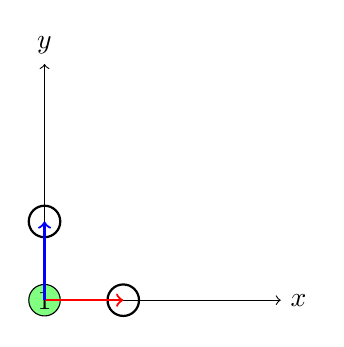
\begin{tikzpicture}
        % Draw axes
        \draw[->] (0,0) -- (3,0) node[right] {$x$};
        \draw[->] (0,0) -- (0,3) node[above] {$y$};

        % Mark origo and label it
        
         \draw[fill=green!50] (0,0) circle (0.2) node {1};

        % Draw empty circles at (1,0) and (0,1)
        \draw[thick] (1,0) circle (0.2);
        \draw[thick] (0,1) circle (0.2);

        % Draw lines with arrows
        \draw[red, thick, ->] (0,0) -- (1,0);
        \draw[blue, thick, ->] (0,0) -- (0,1);
    \end{tikzpicture} 
\par\end{center}

\noindent\textbf{Kérdés:} {\color{ccqqqq}{Hányféleképpen}} lehet eljutni
bármilyen $Oy$ vagy $Ox$ tengelyen elhelyezkedő pontba? \\
 \textbf{Válasz:} Az $Ox$ és $Oy$ tengely mentén minden rácspontba
$1$-est írunk, hiszen csak egyféleképpen lehetett eljutni ezekbe
a pontokba: 
\begin{itemize}
\item $Ox$ pozitív pontjaira úgy hogy origóból jobbra léptünk, 
\item $Oy$ pozitív pontjaira úgy hogy origóból felfele léptünk. 
\end{itemize}
\begin{center}
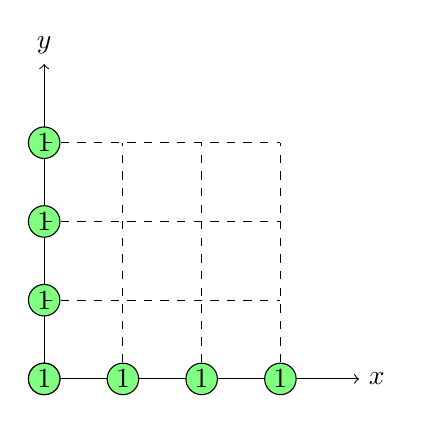
\begin{tikzpicture}
        % Draw axes
        \draw[->] (0,0) -- (4,0) node[right] {$x$};
        \draw[->] (0,0) -- (0,4) node[above] {$y$};

        % Mark points and label them
        \foreach \x in {0,1,2,3} {
            \draw[fill=green!50] (\x,0) circle (0.2) node {1};
            \draw[fill=green!50] (0,\x) circle (0.2) node {1};
        }

        % Grid lines for clarity
        \draw[dashed] (1,0) -- (1,3);
        \draw[dashed] (2,0) -- (2,3);
        \draw[dashed] (3,0) -- (3,3);

        \draw[dashed] (0,1) -- (3,1);
        \draw[dashed] (0,2) -- (3,2);
        \draw[dashed] (0,3) -- (3,3);
    \end{tikzpicture} 
\par\end{center}

\noindent\textbf{Kérdés:} {\color{ccqqqq}{Hogy}} lehet eljutni bármilyen
más pontba, mely nem $Oy$ vagy $Ox$ tengelyen helyezkedik el? \\
 \textbf{Válasz:} Egy adott $(x,y)$ pontba 
\begin{enumerate}
\item tőle \textcolor{red}{balról}, vagyis az $(x-1,y)$ pontból lehet egy
jobbra lépéssel eljutni, 
\item tőle \textcolor{blue}{alulról}, vagyis az $(x,y-1)$ pontból lehet
egy felfele lépéssel eljutni. 
\end{enumerate}
\begin{center}
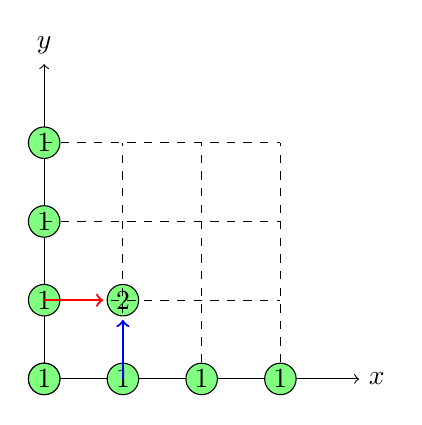
\begin{tikzpicture}
        % Draw axes
        \draw[->] (0,0) -- (4,0) node[right] {$x$};
        \draw[->] (0,0) -- (0,4) node[above] {$y$};

        % Mark points and label them
        \foreach \x in {0,1,2,3} {
            \draw[fill=green!50] (\x,0) circle (0.2) node {1};
            \draw[fill=green!50] (0,\x) circle (0.2) node {1};
        }
        \draw[fill=green!50] (1,1) circle (0.2) node {2};

        % Grid lines for clarity
        \draw[dashed] (1,0) -- (1,3);
        \draw[dashed] (2,0) -- (2,3);
        \draw[dashed] (3,0) -- (3,3);

        \draw[dashed] (0,1) -- (3,1);
        \draw[dashed] (0,2) -- (3,2);
        \draw[dashed] (0,3) -- (3,3);
        
        % Random (x,y) point
        \coordinate (A) at (1,1);

        % Lines from above and from the left
        \draw[red, thick, ->] (0,1) -- (3/4,1);
        \draw[blue, thick, ->] (1,0) -- (1,3/4);
    \end{tikzpicture} 
\par\end{center}

Egy adott $(x,y)$ pontba két különböző úton lehet eljutni: vagy balról,
vagy alulról. Ezért az {\color{ccqqqq}{oda vezető utak száma megegyezik
a balról érkező utak számának és az alulról érkező utak számának összegével.}}

\textbf{A fennebb leírtak alapján az első pár rácspontba a következő
értékek kerülnek:}
\begin{center}
\includegraphics[width=12cm,height=10 cm]{\string"content/Seres_Brigitta_Alexandra/2\string".JPG}
\par\end{center}

\noindent\textbf{Kérdés:} {\color{ccqqqq}{Hányféleképpen}} lehet eljutni
egy $(x,y)$ pontba? \\
 Tudjuk, hogy az $(x,y)$-ba {\color{ccqqqq}{vezető utak száma
megegyezik a balról érkező utak számának és az alulról érkező utak
számának összegével.} }

Ahhoz, hogy végül eljussunk $(x,y)-$ba összesen 
\begin{itemize}
\item $x-$szer kell \textcolor{red}{jobbra (vízszintesen)} lépni, 
\item $y-$szor kell \textcolor{blue}{felfele (függőlegesen)} lépni. 
\end{itemize}
\begin{center}
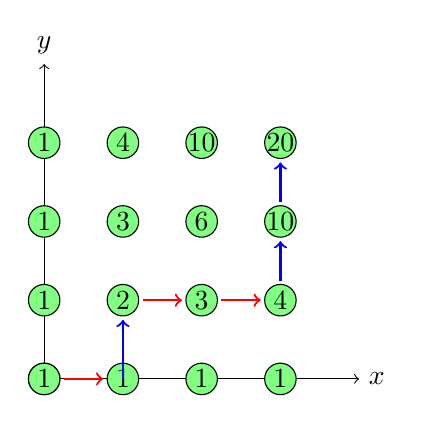
\begin{tikzpicture}
        % Draw axes
        \draw[->] (0,0) -- (4,0) node[right] {$x$};
        \draw[->] (0,0) -- (0,4) node[above] {$y$};

        % Mark points and label them
        \foreach \x in {0,1,2,3} {
            \draw[fill=green!50] (\x,0) circle (0.2) node {1};
            \draw[fill=green!50] (0,\x) circle (0.2) node {1};
        }
        \draw[fill=green!50] (1,1) circle (0.2) node {2};
        \draw[fill=green!50] (1,2) circle (0.2) node {3};
        \draw[fill=green!50] (1,3) circle (0.2) node {4};
        \draw[fill=green!50] (2,1) circle (0.2) node {3};
        \draw[fill=green!50] (2,2) circle (0.2) node {6};
        \draw[fill=green!50] (2,3) circle (0.2) node {10};
        \draw[fill=green!50] (3,1) circle (0.2) node {4};
        \draw[fill=green!50] (3,2) circle (0.2) node {10};
        \draw[fill=green!50] (3,3) circle (0.2) node {20};
        
        % Lines from above and from the left
        \draw[red, thick, ->] (1/4,0) -- (3/4,0);
        \draw[red, thick, ->] (5/4,1) -- (7/4,1);
        \draw[blue, thick, ->] (1,0) -- (1,3/4);
        \draw[red, thick, ->] (9/4,1) -- (11/4,1);
        \draw[blue, thick, ->] (3,5/4) -- (3,7/4);
        \draw[blue, thick, ->] (3,9/4) -- (3,11/4);
    \end{tikzpicture} 
\par\end{center}

Ha le szeretnénk írni egy ilyen útat, elégséges lenne $x+y$ számú
betűt írnunk: 
\begin{itemize}
\item ${\color{red}{v}}$-t minden \textcolor{red}{vízszintes} lépésre, 
\item ${\color{blue}{f}}$-et minden \textcolor{blue}{függőleges} lépésre. 
\end{itemize}
\textbf{Példa.} Egy lehetséges $(3,3)$-ba vezető útat le lehetne
írni \textbf{{\color{red}{v}}{\color{blue}{f}}{\color{red}{v}}{\color{red}{v}}{\color{blue}{f}}{\color{blue}{f}}}
betűsorozattal.

Mivel az $x$ darab $v$ betűt és az $y$ darab $f$ betűt tartalmazó
jelsorozat \textcolor{ccqqqq}{egyértelműen meghatározza az utat
és fordítva}, elégséges az ilyen jelsorozatok számát meghatározni.
Egy jelsorozat egyértelműen meghatározott, ha az $(x+y)$ helyből
kijelölünk $x$ darabot (ide kerülnek a $v$ betűk és a többi helyre
az $f$ betűk). \\
 Ezt ${\color{ccqqqq}{C_{x+y}^{x}}}$ féleképpen tehetjük meg. Tehát
${\color{ccqqqq}{C_{x+y}^{x}}}$ féleképpen lehet eljutni az origóból
$(x,y)$ pontba.

\textbf{Megjegyzés.} Ha a jelsorozatból $y$ darabot választunk ki,
akkor is ugyanezt az eredményt kapjuk meg, szóval igaz, hogy $C_{x+y}^{{\color{blue}{x}}}=C_{x+y}^{{\color{red}{y}}}.$

A fentiek alapján minden $(x,y)$ rácspontba beírható a neki megfelelő
$C_{x+y}^{x}$ kombináció: 
\begin{center}
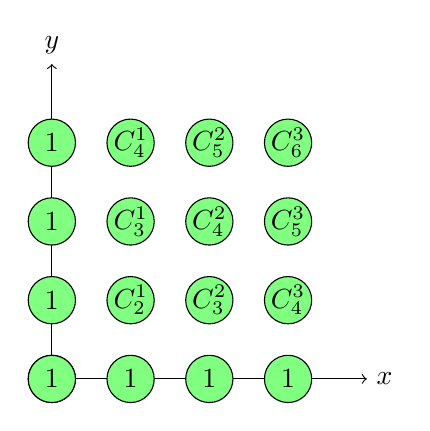
\begin{tikzpicture}
        % Draw axes
        \draw[->] (0,0) -- (4,0) node[right] {$x$};
        \draw[->] (0,0) -- (0,4) node[above] {$y$};

        % Mark points and label them
        \foreach \x in {0,1,2,3} {
            \draw[fill=green!50] (\x,0) circle (0.3) node {1};
            \draw[fill=green!50] (0,\x) circle (0.3) node {1};
        }
        \draw[fill=green!50] (1,1) circle (0.3) node {$C_{2}^{1}$};
        \draw[fill=green!50] (1,2) circle (0.3) node {$C_{3}^{1}$};
        \draw[fill=green!50] (1,3) circle (0.3) node {$C_{4}^{1}$};
        \draw[fill=green!50] (2,1) circle (0.3) node {$C_{3}^{2}$};
        \draw[fill=green!50] (2,2) circle (0.3) node {$C_{4}^{2}$};
        \draw[fill=green!50] (2,3) circle (0.3) node {$C_{5}^{2}$};
        \draw[fill=green!50] (3,1) circle (0.3) node {$C_{4}^{3}$};
        \draw[fill=green!50] (3,2) circle (0.3) node {$C_{5}^{3}$};
        \draw[fill=green!50] (3,3) circle (0.3) node {$C_{6}^{3}$};
        
    \end{tikzpicture} 
\par\end{center}

Amennyiben elfordítjuk a kapott számokat, megkapjuk a \textcolor{ccqqqq}{Pascal-háromszöget.}

\textbf{Pascal-háromszög} 
\[
\begin{array}{rc}
\textbf{0.sor} & \textcolor{red}{1}\\
\textbf{1.sor} & \textcolor{red}{1}\quad\textcolor{red}{1}\\
\textbf{2.sor} & \textcolor{red}{1}\quad2\quad\textcolor{red}{1}\\
\textbf{3.sor} & \textcolor{red}{1}\quad3\quad3\quad\textcolor{red}{1}\\
\textbf{4.sor} & \textcolor{red}{1}\quad4\quad6\quad4\quad\textcolor{red}{1}\\
\textbf{5.sor} & \textcolor{red}{1}\quad5\quad{\color{blue}{10}}\quad{\color{blue}{10}}\quad5\quad\textcolor{red}{1}\\
\textbf{6.sor} & \textcolor{red}{1}\quad6\quad15\quad{\color{blue}{20}}\quad15\quad6\quad\textcolor{red}{1}\\
\textbf{7.sor} & \textcolor{red}{1}\quad7\quad{\color{ccqqqq}{21}}\quad35\quad35\quad{\color{ccqqqq}{21}}\quad7\quad\textcolor{red}{1}\\
\textbf{8.sor} & \textcolor{red}{1}\quad8\quad28\quad56\quad70\quad56\quad28\quad8\quad\textcolor{red}{1}\\
\textbf{9.sor} & \textcolor{red}{1}\quad9\quad36\quad84\quad126\quad126\quad84\quad36\quad9\quad\textcolor{red}{1}\\
\ldots & \ldots\ldots
\end{array}
\]
\textbf{Tulajdonságok:} 
\begin{itemize}
\item Definiálasa végett minden sor első és utolsó eleme ${\color{red}{1}}$-es. 
\item A többi elem a {\color{blue}{fölötte álló két szám összege}},
vagyis teljesül az addiciós képlet: $C_{n}^{k}=C_{n-1}^{k}+C_{n-1}^{k-1},$
ahol $n\geq2$ a sort jelöli és $k$ a pozíciót a sorban, $1\leq k\leq n-1$. 
\item Az $n.$ sorban ${\color{blue}{n+1}}$ elem szerepel. 
\item Az $n.$ sorban szereplő elemek összege ${\color{blue}{2^{n}}}$. 
\item Mivel beláttuk, hogy $C_{x+y}^{x}=C_{x+y}^{y}$, így $C_{x+y}^{x}=C_{x+y}^{x+y-x}$,
vagyis teljesül a szimmetria-tulajdonság, igaz a háromszögben, hogy
{\color{ccqqqq}{a szélektől egyforma távolságra levő számok egymással
egyenlőek.}} 
\end{itemize}
\vspace{0.3cm}

\textbf{JÁTÉK:} Online is elérhető a \textcolor{blue}{\href{https://mathigon.org/course/sequences/pascals-triangle?fbclid=IwY2xjawJSNH1leHRuA2FlbQIxMAABHdKs5VH-uPr_MrJXtm5Bt0-Ima86B7AqARyf5XoyXEeBA_tXzXkG7Vf2Lw_aem_hVcotl8kGh-BhOqF5w-W4g}{Pascal-h\' aromsz\" og}}
kitöltésére vonatkozó játék (lásd \ref{7sb2}-es ábra, megjegyzés:
hasznos eszköz lehet akkor, amikor a diákok még csak ismerkednek a
képzési szabállyal). 
\begin{figure}[h]
\centering \includegraphics[width=10cm,height=6cm]{\string"content/Seres_Brigitta_Alexandra/3\string".JPG}
\caption{Pascal-háromszög kitöltésére vonatkozó online játék}
\label{7sb2}
\end{figure}

\vspace{0.5cm}

\textbf{II. Binomiális együtthatók és Pascal-háromszög közötti kapcsolat}

\vspace{0.3cm}

\begin{center}
% Make the text slightly smaller
\global\long\def\arraystretch{0.9}%
 % Reduce row height
 \setlength{\tabcolsep}{3pt} % Reduce column spacing
 %
\begin{tabular}{ccc}
\textbf{Binom:}  & \textbf{Kifejtés:}  & \textbf{Együtthatók:} \tabularnewline
[3pt] $(a+b)^{0}=$  & $1$  & {\color{red} 1} \tabularnewline
[3pt] $(a+b)^{1}=$  & $a+b$  & {\color{red} 1} \quad{}{\color{red} 1} \tabularnewline
[3pt] $(a+b)^{2}=$  & $a^{2}+{\color{blue}2}ab+b^{2}$  & {\color{red} 1} \quad{}{\color{blue} 2} \quad{}{\color{red}
1} \tabularnewline
[3pt] $(a+b)^{3}=$  & $a^{3}+{\color{magenta}3}a^{2}b+{\color{magenta}3}ab^{2}+b^{3}$  & {\color{red} 1} \quad{}{\color{magenta} 3} \quad{}{\color{magenta}
3} \quad{}{\color{red} 1} \tabularnewline
[3pt] $(a+b)^{4}=$  & $a^{4}+{\color{green}4}a^{3}b+{\color{violet}6}a^{2}b^{2}+{\color{green}4}ab^{3}+b^{4}$  & {\color{red} 1} \quad{}{\color{green} 4} \quad{}{\color{violet}
6} \quad{}{\color{green} 4} \quad{}{\color{red} 1} \tabularnewline
[3pt] $(a+b)^{5}=$  & $a^{5}+{\color{orange}5}a^{4}b+{\color{cyan}10}a^{3}b^{2}+{\color{cyan}10}a^{2}b^{3}+{\color{orange}5}ab^{4}+b^{5}$  & {\color{red} 1} \quad{}{\color{orange} 5} \quad{}{\color{cyan}
10} \quad{}{\color{cyan} 10} \quad{}{\color{orange} 5} \quad{}{\color{red}
1} \tabularnewline
[3pt]  &  & \tabularnewline
\end{tabular}
\par\end{center}

\vspace{0.3cm}

\textbf{Newton binomiális tételének kifejtéséből adódó tagok együtthatói
(binomiális együtthatók) \textcolor{ccqqqq}{megegyeznek} a Pascal-háromszög
megfelelő sorának elemeivel.}

\vspace{0.5cm}

\textbf{III. Érdekességek a Pascal-háromszögben}

\vspace{0.2cm}

\textbf{a.) "Zokni" tulajdonság} \\
 Emlékezzünk vissza, hogy teljesül a \textbf{felső összegzés:} 
\[
\boxed{C_{k}^{{\color{ccqqqq}{k}}}+C_{k+1}^{{\color{ccqqqq}{k}}}+C_{k+2}^{{\color{ccqqqq}{k}}}+\ldots+C_{n}^{{\color{ccqqqq}{k}}}=C_{n+1}^{k+1}},\quad0\leq k\leq n-1.
\]

Ekkor az összegben felsorolt kombinációk alsó indexei változnak $k-$től
$n-$ig, még a felsők \textcolor{ccqqqq}{állandóak}, vagyis a Pascal-háromszögben
soronként megyünk lefele és minden sorból ugyanazzal az indexszámmal
rendelkező elemet válasszuk ki: $k-$adikat, ezeket összegezzük és
ezáltal megkapjuk az $(n+1).$ sor $(k+1).$ elemét.

\textbf{Példa. $k=2$ és $n=7$} 
\[
{\color{blue}{C_{2}^{2}}}+{\color{red}{C_{3}^{2}}}+{\color{violet}{C_{4}^{2}}}+{\color{green}{C_{5}^{2}}}+{\color{cyan}{C_{6}^{2}}}+{\color{ccqqqq}{C_{7}^{2}}}={\color{magenta}{C_{8}^{3}}}
\]
\[
{\color{blue}{1}}+{\color{red}{3}}+{\color{violet}{6}}+{\color{green}{10}}+{\color{cyan}{15}}+{\color{ccqqqq}{21}}={\color{magenta}{56}}
\]

\[
\begin{array}{rc}
\textbf{0.sor} & 1\\
\textbf{1.sor} & 1\quad1\\
\textbf{2.sor} & 1\quad2\quad{\color{blue}{1}}\\
\textbf{3.sor} & 1\quad3\quad{\color{red}{3}}\quad1\\
\textbf{4.sor} & 1\quad4\quad{\color{violet}{6}}\quad4\quad1\\
\textbf{5.sor} & 1\quad5\quad{\color{green}{10}}\quad10\quad5\quad1\\
\textbf{6.sor} & 1\quad6\quad{\color{cyan}{15}}\quad20\quad15\quad6\quad1\\
\textbf{7.sor} & 1\quad7\quad{\color{ccqqqq}{21}}\quad35\quad35\quad21\quad7\quad1\\
\textbf{8.sor} & 1\quad8\quad28\quad{\color{magenta}{56}}\quad70\quad56\quad28\quad8\quad1
\end{array}
\]

\vspace{0.2cm}

\textbf{Honnan ered a név?} A Pascal-háromszög bármely zokni alakú
részében a száron található számok összege az ujjaknál található számmal
egyezik meg (lásd \ref{7sb3}.ábra). 
\begin{figure}[h]
\centering \includegraphics[width=10cm,height=6cm]{\string"content/Seres_Brigitta_Alexandra/4\string".JPG}
\caption{"Zokni" tulajdonság Pascal-háromszögben}
\label{7sb3}
\end{figure}

\textbf{b.) Egy adott sorból a középső elem(ek) a legnagyobb(ak) \label{7sb6}}

\[
\begin{array}{rc}
\textbf{0.sor} & 1\\
\textbf{1.sor} & 1=1\\
\textbf{2.sor} & 1<{\color{red}{2}}>1\\
\textbf{3.sor} & 1<{\color{red}{3=3}}>1\\
\textbf{4.sor} & 1<4<{\color{red}{6}}>4>1\\
\textbf{5.sor} & 1<5<{\color{red}{10=10}}>5>1\\
\textbf{6.sor} & 1<6<15<{\color{red}{20}}>15>6>1\\
\textbf{7.sor} & 1<7<21<{\color{red}{35=35}}>21>7>1\\
\textbf{8.sor} & 1<8<28<56<{\color{red}{70}}>56>28>8>1\\
\textbf{9.sor} & 1<9<36<84<{\color{red}{126=126}}>84>36>9>1\\
\ldots & \ldots\ldots
\end{array}
\]
\textbf{Következtetés:} 
\begin{itemize}
\item Ha $n$ páratlan, akkor a legnagyobb elem a \textcolor{red}{két középső}
lesz, melyek egyenlőek egymással: $C_{n}^{\frac{n-1}{2}}=C_{n}^{\frac{n+1}{2}}$, 
\item Ha $n$ páros, akkor a legnagyobb elem a \textcolor{red}{középső}
lesz: $C_{n}^{\frac{n}{2}}$. 
\end{itemize}

\textbf{c.) Paritás}

\vspace{0.2cm}

\begin{figure}[h]
\centering \includegraphics[width=11cm,height=9cm]{\string"content/Seres_Brigitta_Alexandra/5\string".jpg}
\caption{Paritás szerint színezett Pascal-háromszög}
\label{7sb4} 
\end{figure}

Színezzük ki a Pascal-háromszög első $15$ sorában a számok helyét
paritásuk szerint (lásd \ref{7sb4}.ábra): 
\begin{itemize}
\item \textbf{páros} = {\color{blue}{kék}}, 
\item \textbf{páratlan} = {\color{red}{piros}}. 
\end{itemize}
\begin{enumerate}
\item A Pascal-háromszög mely soraiban áll {\color{blue}{(a szélétől
eltekintve) mindenütt páros}} szám?\\
 \textbf{Válasz:} Azon sorokban, melyben a sor indexe $2^{k}$ alakú.
\item A Pascal-háromszög mely soraiban áll {\color{red}{mindenütt páratlan}}
szám? \textbf{Válasz:} Azon sorokban, melyben a sor indexe $2^{k}-1$
alakú.
\end{enumerate}
\vspace{0.3cm}

\textbf{d.) Fibonacci-sorozat}

Összegezve a Pascal-háromszög átlóit a lennebb megadott szabály szerint
megkapjuk a Fibonacci-sorozat elemeit. 
\begin{figure}[h]
\centering \includegraphics[width=12cm,height=10cm]{\string"content/Seres_Brigitta_Alexandra/6\string".png}
\caption{Fibonacci-sorozat a Pascal-háromszögben}
\label{7sb5} 
\end{figure}

\[
F_{1}=1,\quad F_{2}=1,\quad F_{3}=2,\quad F_{4}=3,\quad F_{5}=5
\]
\[
F_{n+2}=C_{n+1}^{0}+C_{n}^{1}+C_{n-1}^{2}+C_{n-2}^{3}+\ldots=\sum_{j\geq0}C_{n+1-j}^{j}.
\]


\section*{Házi feladatok}
\begin{problem}
Számítsd ki az alábbi összegeket, ahol $k,n\in\mathbb{N}$, $k\leq n$:
\begin{enumerate}
\item[{\small\textbf{a.)}}] ${\displaystyle S_{1}=\sum_{k=0}^{n}2^{k}C_{n}^{k}}$, \quad{}\quad{}\textbf{b.)}
${\displaystyle S_{2}=\sum_{k=0}^{n}kC_{n}^{k}}$,
\item[{\small\textbf{c.)}}] ${\displaystyle S_{3}=1\cdot1!+2\cdot2!+3\cdot3!+\ldots+n\cdot n!.}$ 
\end{enumerate}
\end{problem}

\begin{solution}
\textbf{a.)} Newton binomiális tételében legyen $a=1$ és $b=2$,
ekkor teljesül, hogy 
\[
3^{n}=(1+2)^{n}=\sum_{k=0}^{n}C_{n}^{k}1^{n-k}2^{k}=\sum_{k=0}^{n}2^{k}C_{n}^{k}=S_{1},
\]
tehát $S_{1}=3^{n}$. \\
 \textbf{b.)} Vizsgáljuk meg a $k\cdot C_{n}^{k}$ kifejezést, és
próbáljuk az első tényezőt beolvasztani a $C_{n}^{k}$ kifejezésbe!

\begin{align*}
k\cdot C_{n}^{k} & =k\cdot\frac{n!}{k!(n-k)!}=\frac{n!}{(k-1)!(n-k)!}\\
 & =\frac{n!}{(k-1)![(n-1)-(k-1)]!}=n\cdot\frac{(n-1)!}{(k-1)!(n-k)!}=n\cdot C_{n-1}^{k-1}
\end{align*}
Ezt felhasználva, a kiszámítandó összeget a következőképpen alakíthatjuk:
\begin{align*}
\sum_{k=0}^{n}k\cdot C_{n}^{k} & =\sum_{k=1}^{n}k\cdot C_{n}^{k}=\sum_{k=1}^{n}n\cdot C_{n-1}^{k-1}=n\cdot\sum_{k=1}^{n}C_{n-1}^{k-1}\\
 & =n\cdot\sum_{k=0}^{n-1}C_{n-1}^{k}=n\cdot(C_{n-1}^{0}+C_{n-1}^{1}+C_{n-1}^{2}+\ldots+C_{n-1}^{n-1})=n\cdot2^{n-1}.
\end{align*}
Tehát ${\displaystyle S_{2}=\sum_{k=0}^{n}k\cdot C_{n}^{k}=n\cdot2^{n-1}.}$
\\
 \textbf{c.)} Adjuk hozzá az $S_{3}$ összeghez az $(1!+2!+\ldots+n!)$
összeget: 
\[
S_{3}+(1!+2!+\ldots+n!)=1\cdot1!+2\cdot2!+3\cdot3!+\ldots+n\cdot n!+(1!+2!+\ldots+n!),
\]
ekkor kiemelve a közös tagokat, kapjuk hogy 
\[
S_{3}+(1!+2!+\ldots+n!)=(1+1)\cdot1!+(2+1)\cdot2!+(3+1)\cdot3!+\ldots+(n+1)\cdot n!.
\]
Elvégezve a zárójelek összeadását látható, hogy 
\[
S_{3}+(1!+2!+\ldots+n!)=2\cdot1!+3\cdot2!+4\cdot3!+\ldots+(n+1)\cdot n!,
\]
majd összeszorozva a tagokat: 
\[
S_{3}+(1!+2!+\ldots+n!)=2!+3!+4!+\ldots+n!+(n+1)!.
\]
Az egyenlőség bal és jobb oldalán is megjelenik az $(2!+3!+\ldots+n!)$
összeg, így kivonjuk mindkét oldalból azt, és megkapjuk a keresett
összeget: 
\[
S_{3}+1!=(n+1)!,\quad\text{vagyis}\quad S_{3}=(n+1)!-1.
\]
\end{solution}
\vspace{0.3cm}

\begin{problem}
\textbf{a.)} Határozd meg a racionális tagok darabszámát a következő
binom kifejtéséből $(\sqrt{3}+1)^{12}.$\\
 \textbf{b.)} Határozd meg $a>0$ valós számot, tudva hogy a 
\[
\Big(\sqrt[3]{a}+\frac{1}{\sqrt[4]{a}}\Big)^{12}
\]
binom kifejtésének középső tagja egyenlő $1848$-cal. 
\end{problem}

\begin{solution}
\textbf{a.)} A kifejtés általános tagja, ahol $k\in\{0,1,\ldots,12\}$
\[
T_{k+1}=C_{12}^{k}(\sqrt{3})^{12-k}1^{k}=C_{12}^{k}\cdot3^{\frac{12-k}{2}}.
\]
Egy tag akkor lesz racionális, ha nem tartalmaz irracionális kifejezést
a felírásában. A binomiális együttható mindig egy természetes szám,
így a $3^{\frac{12-k}{2}}$ számnak kell racionálisnak lennie ahhoz,
hogy megfeleljen a feladat kérelmének. Ez akkor történik meg, ha $(12-k)$
osztható $2$-vel, vagyis ha $(12-k)$ páros szám lesz. Mivel $12$
páros szám, a $(12-k)$ kifejezés pontosan akkor lesz páros, ha $k$
páros.

Mivel $k\in\{0,1,2,3,\ldots,12\}$ halmazból lehet, így a megoldás
 $k\in\{0,2,4,6,8,10,12\}$ halmaz lesz, vagyis
ezen értékekre lesz a $T_{k+1}-$es tag racionális. A megoldáshalmaz
számossága egyenlő $7$-el, így elmondható, hogy $7$ darab racionális
tag lesz a $(\sqrt{3}+1)^{12}$ binom kifejtésében.

\vspace{0.1cm}

\textbf{b.)} A kifejtés általános tagja, ahol $k\in\{0,1,\ldots,12\}$
\[
T_{k+1}=C_{12}^{k}(\sqrt[3]{a})^{12-k}{\Big(\frac{1}{\sqrt[4]{a}}\Big)}^{k}=C_{12}^{k}\cdot a^{\frac{12-k}{3}-\frac{k}{4}}.
\]
A kifejtésben $12+1=13$ tag szerepel, ebből a középső tag a $T_{7}$-es
lesz, mert $13$ páratlan szám és egyértelműen meghatározható az $1,2,\ldots,13$
számsorozatból a középső elem, ami a $7$-es lesz. A feltétel szerint
$T_{7}=1848$. Az általános tag képlete alapján tudjuk, hogy $T_{7}$-et
$k=6$-ra kapjuk meg, így igaz, hogy 
\[
T_{7}=C_{12}^{6}\cdot a^{\frac{12-6}{3}-\frac{6}{4}}=C_{12}^{6}\cdot a^{2-\frac{3}{2}}=C_{12}^{6}\cdot a^{\frac{1}{2}}=1848.
\]
Tehát 
\[
924\cdot\sqrt{a}=1848,\quad\text{ahonnan}\quad\sqrt{a}=2,
\]
négyzetre emeléssel megkapjuk, hogy $a=4>0$ a megoldás. 
\end{solution}
\vspace{0.3cm}

\begin{problem}
A Pascal-háromszög tulajdonságai alapján határozd meg, $k$ mely értékére
(értékeire) van maximuma a következő kombinációknak: 
\begin{enumerate}
\item[{\small\textbf{a.)}}] ${\displaystyle C_{24}^{k}}$, \quad{}\quad{}\textbf{b.)} ${\displaystyle C_{13}^{k}}$. 
\end{enumerate}
\end{problem}

\begin{solution}
A Pascal-háromszög előállításából adódóan szimmetrikus, és az értékek
a sorok elején növekednek a szimmetriatengelyig. A legnagyobb elem(ek)
a középső(k) lesz(nek), attól függően, hogy páros vagy páratlan indexű
sorban vagyunk (lásd \ref{7sb6}-es elméleti rész).

\textbf{a.)} Ha páros számnak vett kombinációja érdekel, vagyis páros
indexű sorban vagyunk, a keresett kombináció a maximumát $k=$ a szám
felére veszi fel. Mivel $24$ páros, $k=12$-re veszi fel a ${\displaystyle C_{24}^{k}}$
kombináció a maximumát, vagyis 
\[
C_{24}^{12}=2704156.
\]

\textbf{b.)} Ha páratlan számnak vett kombinációja érdekel, vagyis
páratlan indexű sorban vagyunk, a keresett kombináció a maximumát
két különböző $k$-ra is felveszi, de a maximum értéke ugyanaz lesz.
Ezt a két $k$ értéket úgy kapjuk meg, hogy egyszer a (szám$-1$)
felével lesz egyenlő, majd a (szám$+1$) felével.

Esetünkben $13$ páratlan szám, így a két keresett $k$ érték a 
\[
k_{1}=\frac{13-1}{2}=\frac{12}{2}=6\quad\text{és}\quad k_{2}=\frac{13+1}{2}=\frac{14}{2}=7
\]
számokkal lesz egyenlő. Tehát ${\displaystyle C_{13}^{k}}$ maximumát
$k=6$ és $k=7$ esetén is felveszi, valamint 
\[
C_{13}^{6}=C_{13}^{7}=1716.
\]
\end{solution}
\vspace{0.3cm}

\begin{problem}
Határozd meg az $x^{6}$ együtthatóját az 
\[
(1+x)^{n}+(1+x)^{n-1}
\]
kifejtésében (a tagok összevonása után), ha a kifejtésben megjelenő
binomiális együtthatók összege $1536.$
\end{problem}

\begin{solution}
Newton binomiális tétele alapján 
\begin{align*}
(1+x)^{n}+(1+x)^{n-1} & =\sum_{k=0}^{n}C_{n}^{k}1^{n-k}x^{k}+\sum_{k=0}^{n-1}C_{n-1}^{k}1^{n-1-k}x^{k}\\
 & =\sum_{k=0}^{n}C_{n}^{k}x^{k}+\sum_{k=0}^{n-1}C_{n-1}^{k}x^{k}\\
 & =\sum_{k=0}^{n-1}C_{n}^{k}x^{k}+x^{n}+\sum_{k=0}^{n-1}C_{n-1}^{k}x^{k}\\
 & =\sum_{k=0}^{n-1}(C_{n-1}^{k}+C_{n}^{k})x^{k}+x^{n}.
\end{align*}
A kifejtésben megjelenő binomiális együtthatók összege az ismert összefüggés
szerint 
\[
\sum_{k=0}^{n}C_{n}^{k}+\sum_{k=0}^{n-1}C_{n-1}^{k}=2^{n}+2^{n-1},
\]
ám feltétel szerint a kifejtésben megjelenő binomiális együtthatók
összege $1536$, így $2^{n}+2^{n-1}=1536.$ Mivel $1536=3\cdot2^{9}$,
így $2^{n-1}(2+1)=2^{n-1}\cdot3=3\cdot2^{9}$, vagyis $2^{n-1}=2^{9}$,
ahonnan az exponenciális függvények injektívitása végett $n-1=9$,
tehát $n=10.$

Ekkor $x^{6}$ együtthatója a kifejtésben a tagok összevonása után
\[
C_{9}^{6}+C_{10}^{6}=84+210=294.
\]
\end{solution}
\vspace{0.3cm}

\begin{problem}
\label{7sb8} Lásd be a következő azonosságokat: 
\begin{enumerate}
\item[{\small\textbf{a.)}}] ${\displaystyle C_{n}^{k}\cdot C_{k}^{m}=C_{n}^{m}\cdot C_{n-m}^{k-m},\quad1\leq m\leq k\leq n}$,
\hspace{0.3cm} \textit{(trinomiális alak)}

\vspace{0.3cm}

\item[{\small\textbf{b.)}}] ${\displaystyle \sum_{k=m}^{n}C_{n}^{k}\cdot C_{k}^{m}=C_{n}^{m}\cdot2^{n-m},\quad0\leq m\leq n,}$

\vspace{0.3cm}

\item[{\small\textbf{c.)}}] ${\displaystyle C_{k}^{k}+C_{k+1}^{k}+C_{k+2}^{k}+\ldots+C_{n}^{k}=C_{n+1}^{k+1},\quad0\leq k\leq n-1,}$
\textit{(felső összegzés, "zokni" tulajdonság)}\\
 Mit kapunk az összefüggésből, ha $k=1$?

\vspace{0.3cm}

\item[{\small\textbf{d.)}}] ${\displaystyle \sum_{k=0}^{n}C_{2n}^{k}=2^{2n-1}+\frac{1}{2}C_{2n}^{n},}$

\vspace{0.3cm}

\item[{\small\textbf{e.)}}] ${\displaystyle (C_{n}^{0})^{2}+(C_{n}^{1})^{2}+(C_{n}^{2})^{2}+\ldots+(C_{n}^{n})^{2}=C_{2n}^{n},\quad0\leq n.}$ 
\end{enumerate}
\end{problem}

\begin{solution}
\textbf{Útmutatás:} \textbf{b.)} Használd fel az \textbf{a.)}-t, majd
hajts végre az összegzésben egy indexcserét.\\
 \textbf{c.)} Az addiciós képlet többszöri felhasználása segíthet.\\
 \textbf{d.)} Newton binomiális tétele és a kombinációk szimmetria-tulajdonsága
segíthet.\\
 \textbf{e.)} A Vandermonde-azonosság és a binomiális együtthatók
szimmetria-tulajdonsága segíthet.

\vspace{0.3cm}
 \textbf{a.)} Felhasználjuk a $C_{n}^{k}=\frac{n!}{k!(n-k)!}$ képletet:
\begin{align*}
C_{n}^{k}\cdot C_{k}^{m} & =\frac{n!}{k!(n-k)!}\cdot\frac{k!}{m!(k-m)!}=\frac{n!}{m!(n-k)!(k-m)!}\\
 & =\frac{n!}{m!(n-m)!}\cdot\frac{(n-m)!}{(k-m)!(n-k)!}\\
 & =\frac{n!}{m!(n-m)!}\cdot\frac{(n-m)!}{(k-m)![(n-m)-(k-m)]!}\\
 & =C_{n}^{m}\cdot C_{n-m}^{k-m},\quad\text{ahol}\quad1\leq m\leq k\leq n.
\end{align*}
\textbf{b.)} Felhasználva az \textbf{a.)}-ban belátott trinomiális
alakot, írhatjuk hogy 
\[
{\displaystyle \sum_{k=m}^{n}C_{n}^{k}\cdot C_{k}^{m}={\displaystyle \sum_{k=m}^{n}C_{n}^{m}\cdot C_{n-m}^{k-m},}}
\]
kiemelhetjük az összegből a $C_{n}^{m}$ tagot, hiszen állandó, nem
függ $k$-tól, így 
\[
{\displaystyle \sum_{k=m}^{n}C_{n}^{m}\cdot C_{n-m}^{k-m}={\displaystyle C_{n}^{m}\cdot\sum_{k=m}^{n}C_{n-m}^{k-m}.}}
\]
Az összegzésben bevezetünk egy indexcserét $j=k-m$, így az eredeti
összegünk átírható 
\[
{\displaystyle C_{n}^{m}\cdot\sum_{k=m}^{n}C_{n-m}^{k-m}={\displaystyle C_{n}^{m}\cdot\sum_{j=0}^{n-m}C_{n-m}^{j}=C_{n}^{m}\cdot2^{n-m},}}
\]
ahol az utolsó lépésben felhasználtuk a binomiális együtthatók összegére
vonatkozó képletet. Ezzel beláttuk a kért összefüggést, valóban teljesül,
hogy 
\[
{\displaystyle \sum_{k=m}^{n}C_{n}^{k}\cdot C_{k}^{m}=C_{n}^{m}\cdot2^{n-m},\quad0\leq m\leq n.}
\]

\textbf{c.)} Adjuk össze az addiciós képletből származó következő
egyenlőségeket, ahol $0\leq k\leq n-1$: 
\begin{align*}
C_{n+1}^{k+1} & =C_{n}^{k+1}+C_{n}^{k}\\
C_{n}^{k+1} & =C_{n-1}^{k+1}+C_{n-1}^{k}\\
C_{n-1}^{k+1} & =C_{n-2}^{k+1}+C_{n-2}^{k}\\
 & \ldots\ldots\ldots\\
C_{k+3}^{k+1} & =C_{k+2}^{k+1}+C_{k+2}^{k}\\
C_{k+2}^{k+1} & =C_{k+1}^{k+1}+C_{k+1}^{k}
\end{align*}
Összegezve látható, hogy kiesnek bizonyos tagok (bal oldalon a második
tagtól kezdve mindegyik kiesik a jobb oldali első oszlop tagjaival,
kivéve az utolsót), és ami megmarad az a következőképpen néz ki: 
\[
C_{n+1}^{k+1}=C_{k+1}^{k+1}+C_{n}^{k}+C_{n-1}^{k}+\ldots+C_{k+2}^{k}+C_{k+1}^{k}.
\]
Mivel $C_{k+1}^{k+1}=1=C_{k}^{k}$, így megkaptuk azt, amit a feladat
kért 
\[
C_{n+1}^{k+1}=C_{k}^{k}+C_{k+1}^{k}+C_{k+2}^{k}+\ldots+C_{n-1}^{k}+C_{n}^{k},\quad0\leq k\leq n-1.
\]

\vspace{0.15cm}
 Mit kapunk az összefüggésből, ha $k=1$? Az előbb igazoltak alapján
teljesül: 
\[
C_{1}^{1}+C_{2}^{1}+C_{3}^{1}+\ldots+C_{n-1}^{1}+C_{n}^{1}=C_{n+1}^{2},
\]
amit kibontva megkapjuk a már jól ismert első $n$ pozitív egész számok
összegére vonatkozó képletet: 
\[
1+2+3+\ldots+(n-1)+n=\frac{(n+1)!}{2!(n-1)!}=\frac{n(n+1)}{2}.
\]
\textbf{d.)} Newton binomiális tételében ha $a=b=1$, akkor 
\[
(1+1)^{2n}=2^{2n}=\sum_{k=0}^{2n}C_{2n}^{k}.
\]
Mivel $2n$ páros szám, bármilyen $n$ értékre, így az összeg kifejtésében
páratlan darabnyi elem szerepel: $2n+1$. Ekkor kibontjuk az összeget,
egymás alá írva a kombinációk szimmetria-tulajdonsága (${\displaystyle C_{n}^{k}=C_{n}^{n-k}}$)
alapján egymással megegyező tagokat, és középen lesz egy tag pár nélkül.
\begin{align*}
2^{2n}=\sum_{k=0}^{2n}C_{2n}^{k} & =C_{2n}^{0}+C_{2n}^{1}+\ldots+C_{2n}^{n-1}+C_{2n}^{n}+\\
 & +C_{2n}^{2n}+C_{2n}^{2n-1}+\ldots+C_{2n}^{n+1}.
\end{align*}
Az egymással megegyező tagokat összevonjuk, így 
\[
2^{2n}=\sum_{k=0}^{2n}C_{2n}^{k}=2\cdot(C_{2n}^{0}+C_{2n}^{1}+\ldots+C_{2n}^{n-1})+C_{2n}^{n}.
\]
Tehát 
\[
2^{2n}=2\cdot\sum_{k=0}^{n-1}C_{2n}^{k}+(2-1)C_{2n}^{n}=2\cdot\sum_{k=0}^{n}C_{2n}^{k}-C_{2n}^{n},
\]
amit végigosztva $2$-vel és átrendezve, megkapjuk amit bizonyítani
kellett: 
\[
2^{2n-1}=\sum_{k=0}^{n}C_{2n}^{k}-\frac{1}{2}C_{2n}^{n}\quad\iff\quad\sum_{k=0}^{n}C_{2n}^{k}=2^{2n-1}+\frac{1}{2}C_{2n}^{n}.
\]
\textbf{e.)} Ismert a Vandermonde-azonosság: 
\[
C_{m}^{{\color{red}{0}}}\cdot C_{n}^{{\color{blue}{r}}}+C_{m}^{{\color{red}{1}}}\cdot C_{n}^{{\color{blue}{r-1}}}+C_{m}^{{\color{red}{2}}}\cdot C_{n}^{{\color{blue}{r-2}}}+\ldots+C_{m}^{{\color{red}{r}}}\cdot C_{n}^{{\color{blue}{0}}}=C_{m+n}^{r},
\]
\[
0\leq r,\quad r\leq m,\quad r\leq n.
\]
A Vandermonde-azonosságban legyen $m=n$ és $r=n$, ekkor azt kapjuk,
hogy 
\[
C_{n}^{0}\cdot C_{n}^{n}+C_{n}^{1}\cdot C_{n}^{n-1}+C_{n}^{2}\cdot C_{n}^{n-2}+\ldots+C_{n}^{n}\cdot C_{n}^{0}=C_{n+n}^{n}.
\]
A binomiális együtthatók szimmetria-tulajdonsága alapján (${\displaystyle C_{n}^{k}=C_{n}^{n-k}}$)
írható, hogy 
\[
C_{n}^{0}\cdot C_{n}^{0}+C_{n}^{1}\cdot C_{n}^{1}+C_{n}^{2}\cdot C_{n}^{2}+\ldots+C_{n}^{n}\cdot C_{n}^{n}=C_{2n}^{n},
\]
vagyis megkapjuk amit bizonyítani kellett 
\[
{\displaystyle (C_{n}^{0})^{2}+(C_{n}^{1})^{2}+(C_{n}^{2})^{2}+\ldots+(C_{n}^{n})^{2}=C_{2n}^{n},\quad0\leq n.}
\]
\end{solution}
\vspace{0.3cm}

\begin{problem}
Számítsd ki a kért összeget, majd bizonyítsd be a kért azonosságot: 
\begin{itemize}
\item[{\small\textbf{a.)}}] ${\displaystyle S_{1}=\sum_{k=1}^{n}k^{2}C_{n}^{k}}$, \quad{}\quad{}\textbf{b.)}
${\displaystyle 2\cdot\sum_{k=0}^{m-2}C_{m-1}^{k}\cdot C_{m-1}^{k+1}=\frac{m-1}{2m-1}\cdot C_{2m}^{m}.}$
\end{itemize}
\end{problem}

\begin{solution}
\textbf{a.)} Többszörösen felhasználjuk a ${\displaystyle C_{n}^{k}=\frac{n!}{k!(n-k)!}}$
képletet: 
\begin{align*}
S_{1} & =\sum_{k=1}^{n}k^{2}C_{n}^{k}=\sum_{k=1}^{n}k^{2}\cdot\frac{n!}{k!(n-k)!}\\
 & =\sum_{k=1}^{n}k^{2}\cdot\frac{n}{k}\cdot\frac{(n-1)!}{(k-1)![(n-1)-(k-1)]!}=\sum_{k=1}^{n}k^{2}\cdot\frac{n}{k}\cdot C_{n-1}^{k-1}
\end{align*}
Kiemelhetjük az $n$-t, hiszen állandó: 
\[
S_{1}=n\sum_{k=1}^{n}kC_{n-1}^{k-1}.
\]
Továbbá 
\[
S_{1}=n\sum_{k=1}^{n}(k-1+1)C_{n-1}^{k-1}=n\sum_{k=1}^{n}(k-1)C_{n-1}^{k-1}+n\sum_{k=1}^{n}C_{n-1}^{k-1}.
\]
A második tagban szereplő összeg eredményét ismerjük a binomiális
együtthatók összegképletéből, így írható, hogy 
\[
S_{1}=n\sum_{k=1}^{n}(k-1)C_{n-1}^{k-1}+n\cdot2^{n-1}.
\]
Továbbá 
\begin{align*}
S_{1} & =n\sum_{k=1}^{n}(k-1)\cdot\frac{(n-1)!}{(k-1)!(n-k)!}+n\cdot2^{n-1}\\
 & =n\sum_{k=2}^{n}(n-1)\cdot\frac{(n-2)!}{(k-2)!(n-k)!}+n\cdot2^{n-1}\\
 & =n(n-1)\sum_{k=2}^{n}C_{n-2}^{k-2}+n\cdot2^{n-1}.
\end{align*}
Az első tagban szereplő összeg eredményét ismerjük a binomiális együtthatók
összegképletéből, így írható, hogy 
\begin{align*}
S_{1} & =n(n-1)\cdot2^{n-2}+n\cdot2^{n-1}\\
 & =n\cdot2^{n-2}(n-1+2)=n(n+1)\cdot2^{n-2}.
\end{align*}
Tehát a keresett összeg eredménye 
\[
S_{1}=\sum_{k=1}^{n}k^{2}C_{n}^{k}=n(n+1)2^{n-2}.
\]
\textbf{b.)} A binomiális együtthatók szimmetria-tulajdonsága (${\displaystyle C_{n}^{k}=C_{n}^{n-k}}$)
alapján írható, hogy 
\[
\sum_{k=0}^{m-2}C_{m-1}^{k}C_{m-1}^{k+1}=\sum_{k=0}^{m-2}C_{m-1}^{k}C_{m-1}^{(m-1)-(k+1)}=\sum_{k=0}^{m-2}C_{m-1}^{k}C_{m-1}^{m-k-2}.
\]
Továbbá a Vandermonde-azonosság végett igaz, hogy 
\[
\sum_{k=0}^{m-2}C_{m-1}^{k}C_{m-1}^{m-k-2}=C_{m-1+m-1}^{m-2}=C_{2m-2}^{m-2}.
\]
Másrészt 
\[
2\cdot\frac{2m-1}{m-1}\cdot C_{2m-2}^{m-2}=2\cdot\frac{2m-1}{m-1}\cdot\frac{(2m-2)!}{(m-2)!m!}=2\cdot\frac{(2m-1)!}{(m-1)!m!}=2C_{2m-1}^{m-1}.
\]
Felhasználva a binomiális együtthatók szimmetria-tulajdonságát (${\displaystyle C_{n}^{k}=C_{n}^{n-k}}$),
majd az addiciós képletet, kapjuk hogy 
\[
2C_{2m-1}^{m-1}=C_{2m-1}^{2m-1-(m-1)}+C_{2m-1}^{m-1}=C_{2m-1}^{m}+C_{2m-1}^{m-1}=C_{2m}^{m}.
\]
Összegezve 
\[
2\sum_{k=0}^{m-2}C_{m-1}^{k}C_{m-1}^{k+1}=2\cdot C_{2m-2}^{m-2}=\frac{m-1}{2m-1}\cdot2C_{2m-1}^{m-1}=\frac{m-1}{2m-1}C_{2m}^{m},
\]
vagyis beláttuk amit a feladat kért. 
\end{solution}
\vspace{0.3cm}

\begin{problem}
Az alábbi háromszög képzési szabálya ugyanaz, mint a Pascal háromszögnek
(az $(n+1)$-edik sor $k$ indexű elemét az $n-$edik sor $(k-1)$
és $k$ indexű elemének összegéből kapjuk meg, ahol $1\leq k\leq n-2$,
ha $0$-tól indexelünk egy adott sorban), csak az $n$-edik sor első
és utolsó eleme minden $n\geq1$-re éppen $n$. Határozd meg az $n$-edik
sor $k$-adik elemének képletét (sejtésed igazold is)! 
\[
\begin{array}{rc}
\textbf{1.sor} & 1\\
\textbf{2.sor} & 2\quad2\\
\textbf{3.sor} & 3\quad4\quad3\\
\textbf{4.sor} & 4\quad7\quad7\quad4\\
\textbf{5.sor} & 5\quad11\quad14\quad11\quad5\\
\textbf{6.sor} & 6\quad16\quad25\quad25\quad16\quad6\\
\ldots & \ldots\ldots
\end{array}
\]
\end{problem}

\begin{solution}
A mellékelt ábrán látható, hogy az első Pascal-háromszög külső elemeit
elhagyva és a maradék táblázat minden eleméből kivonva a jobb oldalon
látható Pascal-háromszög megfelelő elemét (két sorral lennebb tolva
van megadva) éppen a vizsgált háromszöghöz jutunk. 
\begin{center}
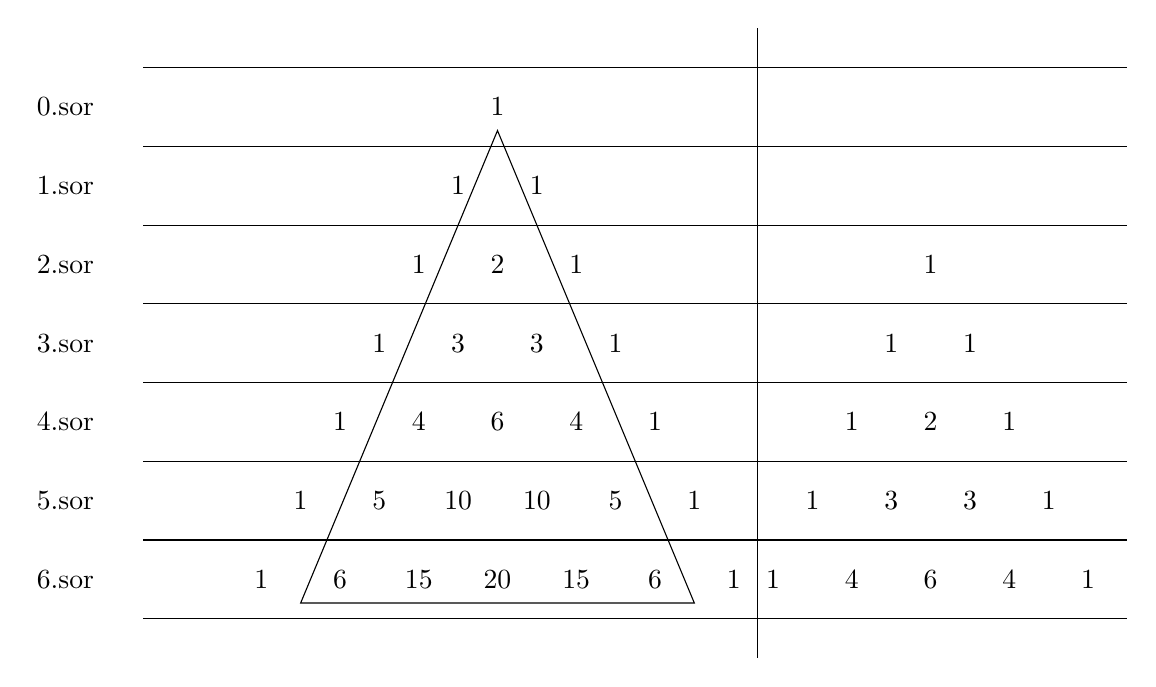
\begin{tikzpicture}[scale=1]

    % Horizontal lines (on integers)
    \foreach \y in {0,...,7} {
        \draw (-4.5, -\y) -- (8, -\y);
    }

    % Vertical dividing line - nudged right to avoid overlapping numbers
    \draw (3.3, 0.5) -- (3.3, -7.5);

    % Left Pascal's triangle (rows 0 to 6), numbers centered between lines
    \foreach \n in {0,...,6} {
        \foreach \k in {0,...,\n} {
            \pgfmathsetmacro{\binom}{int(factorial(\n)/(factorial(\k)*factorial(\n-\k)))}
            \node at (-\n/2+\k, -\n - 0.5) {\binom};
        }
    }

    % Right Pascal's triangle (rows 0 to 4), shifted down by 2 rows
    \foreach \n in {0,...,4} {
        \foreach \k in {0,...,\n} {
            \pgfmathsetmacro{\binom}{int(factorial(\n)/(factorial(\k)*factorial(\n-\k)))}
            \node at (5.5 + \k - \n/2, -\n - 2.5) {\binom};
        }
    }

    % Lowered ^-shaped triangle outline (offset by 0.3)
    \draw (0, -0.8) -- (-2.5, -6.8) -- (2.5, -6.8) -- cycle;

    % Row labels: 0.sor to 6.sor
    \foreach \n in {0,...,6} {
        \node[anchor=east] at (-5, -\n - 0.5) {\n.sor};
    }

\end{tikzpicture} 
\par\end{center}
Az általunk vizsgált háromszög $n$-edik sorában pontosan $n$ darab
elem van, $0$-tól $(n-1)$-ig indexelve.

Sejtésünk az, hogy az általunk vizsgált háromszög $n$-edik sorának
$k$-adik elemét a következőképpen kapjuk meg, ahol $0\leq k\leq n-1$:
\[
C_{n+1}^{k+1}-C_{n-1}^{k}.
\]
Sejtésünk matematikai indukcióval látjuk be.

\textbf{I. Ellenőrzés:} $n=1$ esetén $k=0$ lehet csak, ekkor 
\[
C_{1+1}^{0+1}-C_{1-1}^{0}=C_{2}^{1}-C_{0}^{0}=2-1=1,
\]
valóban megegyezik a mi háromszögünk első sorának egyetlen elemével.

$n=2$ esetén $k=0$ vagy $k=1$ lehet csak, ekkor 
\[
C_{2+1}^{0+1}-C_{2-1}^{0}=C_{3}^{1}-C_{1}^{0}=3-1=2,
\]
és 
\[
C_{2+1}^{1+1}-C_{2-1}^{1}=C_{3}^{2}-C_{1}^{1}=3-1=2,
\]
valóban megegyezik a mi háromszögünk második sorának két elemével.

$n=3$ esetén $k\in\{0,1,2\}$ lehet, ekkor 
\[
C_{3+1}^{0+1}-C_{3-1}^{0}=C_{4}^{1}-C_{2}^{0}=4-1=3,
\]
és 
\[
C_{3+1}^{1+1}-C_{3-1}^{1}=C_{4}^{2}-C_{2}^{1}=6-2=4,
\]
és 
\[
C_{3+1}^{2+1}-C_{3-1}^{2}=C_{4}^{3}-C_{2}^{2}=4-1=3.
\]
Valóban megegyezik a mi háromszögünk harmadik sorának elemeivel.

\vspace{0.15cm}

\textbf{II. Indukciós feltevés:} Tegyük fel, hogy az általunk vizsgált
háromszög $n$-edik sorának $k$-adik elemét a $C_{n+1}^{k+1}-C_{n-1}^{k}$
képlettel kapjuk meg, ahol $0\leq k\leq n-1$.

Lássuk be, hogy az $(n+1)$-edik sor $k$-adik elemének képlete $C_{n+2}^{k+1}-C_{n}^{k}$,
ahol $0\leq k\leq n$.

Az általunk vizsgált háromszögben a Pascal-háromszög képzési szabálya
érvényes, így tudjuk, hogy az $(n+1)$-edik sor $k$ indexű elemét
(jelöljük $x$-el) az $n-$edik sor $(k-1)$ és $k$ indexű elemének
összegéből kapjuk meg. Az indukciós feltevés szerint ekkor igaz, hogy
\[
x=(C_{n+1}^{k-1+1}-C_{n-1}^{k-1})+(C_{n+1}^{k+1}-C_{n-1}^{k}),
\]
vagyis 
\[
x=C_{n+1}^{k}-C_{n-1}^{k-1}+C_{n+1}^{k+1}-C_{n-1}^{k}.
\]
Ekkor 
\[
x=(C_{n+1}^{k}+C_{n+1}^{k+1})-(C_{n-1}^{k-1}+C_{n-1}^{k}).
\]
A kombinációk addiciós képletéből tudjuk, hogy $C_{n}^{k}=C_{n-1}^{k}+C_{n-1}^{k-1}$,
ezt felhasználva, írható, hogy 
\[
x=C_{n+2}^{k+1}-C_{n}^{k},
\]
amit bizonyítani szerettünk volna, ahol $1\leq k\leq n-1.$

Az $(n+1)$-edik sor két szélén levő elemek a képzési szabály szerint
egyenlőek $(n+1)$-el. Ezek a $k=0$-ás és $k=n$-es indexű elemek.
Kérdés, hogy $C_{n+2}^{k+1}-C_{n}^{k}$ képlet esetükben is visszaadja-e
azt, amit a képzési szabály elmond a két elemről?

$k=0$ esetén $C_{n+2}^{1}-C_{n}^{0}=n+2-1=n+1,$ és $k=n$ esetén
$C_{n+2}^{n+1}-C_{n}^{n}=n+2-1=n+1,$ vagyis valóben mindkét szélső
számra is teljesül a képlet, ugyanazt az értéket adja vissza, mint
amit a képzési szabály elmond róluk.

Összességében beláttuk, hogy az $(n+1)$-edik sor minden elemét meg
tudjuk adni a $C_{n+2}^{k+1}-C_{n}^{k}$ képlettel, ahol $0\leq k\leq n$.

\vspace{0.15cm}

\textbf{III. Következtetés:} A matematikai indukció elve alapján igaz,
hogy az az általunk vizsgált háromszög $n$-edik sorának $k$-adik
elemét a $C_{n+1}^{k+1}-C_{n-1}^{k}$ képlettel kapjuk meg, ahol $0\leq k\leq n-1$. 
\end{solution}

\section*{Nehezebb feladatok}
\begin{extraproblem}[Csurka-Molnár Hanna]
Igazoljuk az alábbi összefüggést! 
\[
\sum_{k=0}^{2m}(-1)^{k}C_{4m}^{2k}=(-4)^{m}
\]
\end{extraproblem}

\begin{solution}
Az összefüggés $m=0$ esetén $C_{0}^{0}=(-4)^{0}$ alakú, ami igaz,
mert $1=1$. Vizsgáljuk $1<m$ értékek esetén az összefüggést.

A Pascal-háromszög elemei közti összefüggés alapján tudjuk, hogy 
\begin{equation}
C_{n}^{k}=C_{n-1}^{k-1}+C_{n-1}^{k}\quad\forall\;n,k\in\mathbb{N}^{*}.
\end{equation}
Ez alapján a Pascal-háromszög egy sorának két egymás utáni elemének
összege: 
\begin{align}
C_{n}^{k}-C_{n}^{k+1} & =\left(C_{n-1}^{k-1}+C_{n-1}^{k}\right)-\left(C_{n-1}^{k}+C_{n-1}^{k+1}\right)\nonumber \\
C_{n}^{k}-C_{n}^{k+1} & =C_{n-1}^{k-1}-C_{n-1}^{k+1}\quad\forall\;n,k\in\mathbb{N}^{*}.
\end{align}
A bizonyítandó összefüggésben szereplő összeg a Pascal-háromszög $4m$-ik
sorából származó elemekből áll. Az előbbiekben felírt összefüggéseket
felhasználva felírjuk az összeget a Pascal-háromszög $4m-1$-ik sorából
származó elemek függvényében: 
\begin{align*}
\sum_{k=0}^{2m}(-1)^{k}C_{4m}^{2k}= & C_{4m}^{0}+\sum_{k=1}^{2m-1}(-1)^{k}C_{4m}^{2k}+C_{4m}^{4m}=\\
= & C_{4m-1}^{0}+\sum_{k=1}^{2m-1}(-1)^{k}\left(C_{4m-1}^{2k-1}+C_{4m-1}^{2k}\right)+C_{4m-1}^{4m-1}=\\
= & C_{4m-1}^{0}+\sum_{k=1}^{2m-1}(-1)^{k}C_{4m-1}^{2k}+\sum_{k=1}^{2m-1}(-1)^{k}C_{4m-1}^{2k-1}+C_{4m-1}^{4m-1}=\\
= & \sum_{k=0}^{2m-1}(-1)^{k}C_{4m-1}^{2k}+\sum_{k=1}^{2m}(-1)^{k}C_{4m-1}^{2k-1}=\\
= & \sum_{k=0}^{2m-1}(-1)^{k}C_{4m-1}^{2k}+\sum_{k=0}^{2m-1}(-1)^{k+1}C_{4m-1}^{2k+1}=\\
= & \sum_{k=0}^{2m-1}(-1)^{k}\left(C_{4m-1}^{2k}-C_{4m-1}^{2k+1}\right)
\end{align*}
Ezt a $4m-1$-ik sorból származó elemekből alkotott összeget felírjuk
a $4m-2$-ik sor elemeinek a függvényében: 
\begin{align*}
\sum_{k=0}^{2m-1} & (-1)^{k}\left(C_{4m-1}^{2k}-C_{4m-1}^{2k+1}\right)=\\
= & C_{4m-1}^{0}-C_{4m-1}^{1}+\sum_{k=1}^{2m-2}(-1)^{k}\left(C_{4m-1}^{2k}-C_{4m-1}^{2k+1}\right)-\left(C_{4m-1}^{4m-2}-C_{4m-1}^{4m-1}\right)=\\
= & C_{4m-2}^{0}-\left(C_{4m-2}^{0}+C_{4m-2}^{1}\right)\\
 & +\sum_{k=1}^{2m-2}(-1)^{k}\left[\left(C_{4m-2}^{2k-1}+C_{4m-2}^{2k}\right)-\left(C_{4m-2}^{2k}+C_{4m-2}^{2k+1}\right)\right]\\
 & -\left[\left(C_{4m-2}^{4m-3}+C_{4m-2}^{4m-2}\right)-C_{4m-2}^{4m-2}\right]=\\
= & -C_{4m-2}^{1}+\sum_{k=1}^{2m-2}(-1)^{k}\left(C_{4m-2}^{2k-1}-C_{4m-2}^{2k+1}\right)-C_{4m-2}^{4m-3}=\\
= & -(-1)^{0}C_{4m-2}^{2\cdot0+1}-\sum_{k=1}^{2m-2}(-1)^{k}C_{4m-2}^{2k+1}\\
 & +\sum_{k=1}^{2m-2}(-1)^{k}C_{4m-2}^{2k-1}+(-1)^{2m-1}C_{4m-2}^{2(2m-1)-1}=\\
= & -\sum_{k=0}^{2m-2}(-1)^{k}C_{4m-2}^{2k+1}+\sum_{k=1}^{2m-1}(-1)^{k}C_{4m-2}^{2k-1}=\\
= & -\sum_{k=0}^{2m-2}(-1)^{k}C_{4m-2}^{2k+1}+\sum_{k=0}^{2m-2}(-1)^{k+1}C_{4m-2}^{2k+1}=\\
= & -2\sum_{k=0}^{2m-2}(-1)^{k}C_{4m-2}^{2k+1}
\end{align*}
A fenti összeg $-2$ szorzótényezőjét elhagyva tovább alakítjuk a
$4m-2$-ik sor elemeiből álló összeget, hogy csak a $4m-3$-ik, majd
csak a $4m-4$-ik sor elemei szerepeljenek benne: 
\begin{align*}
\sum_{k=0}^{2m-2}(-1)^{k}C_{4m-2}^{2k+1}= & \sum_{k=0}^{2m-2}(-1)^{k}\left(C_{4m-3}^{2k}+C_{4m-3}^{2k+1}\right)=\\
= & \sum_{k=0}^{2m-2}(-1)^{k}C_{4m-3}^{2k}+\sum_{k=0}^{2m-2}(-1)^{k}C_{4m-3}^{2k+1}=\\
= & C_{4m-3}^{0}+\sum_{k=1}^{2m-2}(-1)^{k}C_{4m-3}^{2k}+\sum_{k=0}^{2m-3}(-1)^{k}C_{4m-3}^{2k+1}+C_{4m-3}^{4m-3}=\\
= & C_{4m-3}^{0}+\sum_{k=0}^{2m-3}(-1)^{k+1}C_{4m-3}^{2k+2}+\sum_{k=0}^{2m-3}(-1)^{k}C_{4m-3}^{2k+1}+C_{4m-3}^{4m-3}=\\
= & C_{4m-3}^{0}+\sum_{k=0}^{2m-3}(-1)^{k}\left(C_{4m-3}^{2k+1}-C_{4m-3}^{2k+2}\right)+C_{4m-3}^{4m-3}=\\
= & C_{4m-4}^{0}\\
 & +\sum_{k=0}^{2m-3}(-1)^{k}\left[\left(C_{4m-4}^{2k}+C_{4m-4}^{2k+1}\right)-\left(C_{4m-4}^{2k+1}+C_{4m-4}^{2k+2}\right)\right]\\
 & +C_{4m-4}^{4m-4}=\\
= & C_{4m-4}^{0}+\sum_{k=0}^{2m-3}(-1)^{k}\left(C_{4m-4}^{2k}-C_{4m-4}^{2k+2}\right)+C_{4m-4}^{4m-4}=\\
= & C_{4m-4}^{0}+\sum_{k=0}^{2m-3}(-1)^{k+1}C_{4m-4}^{2k+2}+\sum_{k=0}^{2m-3}(-1)^{k}C_{4m-4}^{2k}+C_{4m-4}^{4m-4}=\\
= & C_{4m-4}^{0}+\sum_{k=1}^{2m-2}(-1)^{k}C_{4m-4}^{2k}\\
 & +\sum_{k=0}^{2m-3}(-1)^{k}C_{4m-4}^{2k}+(-1)^{4m-4}C_{4m-4}^{2(2m-2)}=\\
= & 2\sum_{k=0}^{2m-2}(-1)^{k}C_{4m-4}^{2k}
\end{align*}

Összegezve a fenti számításokat a következő összefüggést kapjuk: 
\[
\sum_{k=0}^{2m}(-1)^{k}C_{4m}^{2k}=-4\sum_{k=0}^{2m-2}(-1)^{k}C_{4m-4}^{2k}
\]

Tekintsük a következő állítást: 
\[
P(m):\sum_{k=0}^{2m}(-1)^{k}C_{4m}^{2k}=(-4)^{m}
\]
Láttuk, hogy $P(0)$ igaz. Feltételezzük, hogy $P(k)$ igaz $\forall k<m$
egy rögzített $m\in\mathbb{N}$ érték esetén. Ekkor 
\[
\sum_{k=0}^{2m}(-1)^{k}C_{4m}^{2k}=-4\sum_{k=0}^{2m-2}(-1)^{k}C_{4m-4}^{2k}=-4\cdot(-4)^{m-1}=(-4)^{m}
\]
tehát $P(m+1)$ is igaz. A matematikai indukció alapján $P(m)$ igaz
$\forall m\in\mathbb{N}$, tehát igazoltuk az összefüggést. 
\end{solution}
\begin{extraproblem}[Czofa Vivien]
Bizonyítsuk be, hogy az $\left\lfloor (2+\sqrt{3})^{n}\right\rfloor $
páratlan szám, minden $n\in\mathbb{N}^{*}$ esetén!
\end{extraproblem}

\begin{solution}
Alkalmazva Newton binomiális tételét, a következőt írhatjuk:

\[
(2+\sqrt{3})^{n}=\sum_{k=0}^{n}\binom{n}{k}2^{n-k}\cdot(\sqrt{3})^{k}=a_{n}+b_{n}\sqrt{3},\quad a_{n},b_{n}\in\mathbb{N}
\]

Innen, alkalmazva az egész rész valamint a binomiális kifejtés tulajdonságait,
írható:

\[
\left\lfloor (2+\sqrt{3})^{n}\right\rfloor =[a_{n}+b_{n}\cdot\sqrt{3}]=[2a_{n}-(a_{n}-b_{n}\sqrt{3})]=[2a_{n}-(2-\sqrt{3})^{n}]=2a_{n}+\left\lfloor -(2-\sqrt{3})^{n}\right\rfloor 
\]

Az $\left\lfloor -(2-\sqrt{3})^{n}\right\rfloor $ érték meghatározható
a következő módon:

\[
0<2-\sqrt{3}<1\Rightarrow0<(2-\sqrt{3})^{n}<1,\quad\forall n\in\mathbb{N}^{*}\Rightarrow-1<-(2-\sqrt{3})^{n}<0,\quad\forall n\in\mathbb{N}^{*}\Rightarrow\left\lfloor -(2-\sqrt{3})^{n}\right\rfloor =-1
\]

\bigskip{}

\textbf{Összegezve:}

\[
\forall n\in\mathbb{N}^{*},\exists a_{n}\in\mathbb{N}:\left\lfloor (2+\sqrt{3})^{n}\right\rfloor =2a_{n}-1
\]

Vagyis $\left\lfloor (2+\sqrt{3})^{n}\right\rfloor $ páratlan szám,
minden $n\in\mathbb{N}^{*}$ esetén.
\end{solution}
\begin{extraproblem}[Czofa Vivien]
Legyen $m\in\mathbb{N}^{*}$ tetszőlegesen rögzített. Számítsuk ki
az alábbi összeget:
\[
S=1\cdot2\cdot3\cdots m+2\cdot3\cdots(m+1)+\ldots+n(n+1)\cdots(n+m-1).
\]
\end{extraproblem}
\begin{solution}
Az összeg általános tagja $k(k+1)\cdots(k+m-1)$, ahol $k=1,\overline{n}$.

Kiegészítve a faktoriálist kapjuk, hogy: 
\[
k(k+1)\cdots(k+m-1)=\frac{(k+m-1)!}{(k-1)!}=m!\binom{k+m-1}{m}.
\]

Így $S$ átírható az alábbi alakba: 
\[
S=m!\left(\binom{m}{m}+\binom{m+1}{m}+\binom{m+2}{m}+\ldots+\binom{m+n-1}{m}\right).
\]

Emlékezzünk a Pascal-egyenlőségre kombinációk esetén, vagyis: 
\[
\binom{b}{a}=\binom{b-1}{a}+\binom{b-1}{a-1},\quad\forall a,b\in\mathbb{N},a>b.
\]

Választva $a=m$, $b=k+m$, ahol $k>1$, kapjuk, hogy: 
\[
\binom{m+k}{m}=\binom{m+k-1}{m}+\binom{m+k-1}{m-1},\quad\forall k=2,\overline{n}.
\]

Felhasználva még, hogy $\binom{m+n}{m}=\binom{m+n-1}{m}+\binom{m+n-1}{m-1}$,
írhatjuk, hogy:

\[
S=m!\left(\binom{m+1}{m+1}-\binom{m+1}{m}+\binom{m+2}{m+1}-\binom{m+2}{m}+\ldots+\binom{m+n}{m+1}-\binom{m+n}{m}\right).
\]

A megfelelő tagok kiesése után kapjuk, hogy:

\[
S=m!\binom{m+n}{m+1}=m!\cdot\frac{n(n+1)\cdots(n+m)}{m+1}.
\]

\bigskip{}

\textbf{Tehát:}

\[
1\cdot2\cdot3\cdots m+2\cdot3\cdots(m+1)+\ldots+n(n+1)\cdots(n+m-1)=\frac{n(n+1)\cdots(n+m)}{m+1}.
\]
\end{solution}
\begin{extraproblem}[Gál Tamara]
Számítsd ki az $S_{n}=\sum_{k=0}^{n}(-1)^{k}\cdot C_{n}^{k}\cdot C_{3n-k}^{n}$
összeget! \emph{(Megyei olimpia, 1997, Maros megye)}
\end{extraproblem}

\begin{solution}
Az $(1+x)^{3n-k}$ kifejtésében, $x^{n}$ együtthatója $C_{3n-k}^{n}$
tehát $(-1)^{k}C_{n}^{k}C_{3n-k}^{n}$ az $x^{n}$ együtthatója $(-1)^{k}C_{n}^{k}(1+x)^{3n-k}$
összegben. Másrészt 
\[
\sum_{k=0}^{n}=(-1)^{k}C_{n}^{k}(1+x)^{3n-k}=(1+x)^{2n}\sum_{k=0}^{n}=(-1)^{k}C_{n}^{k}(1+x)^{n-k}
\]
\[
=(1+x)^{2}n\cdot((1+x)-1)^{n}=x^{n}(1+x)^{2n},
\]
Tehát $x^{n}$ együtthatója 1 lesz. 
\end{solution}
\begin{extraproblem}[Gál Tamara]
A Pascal háromszög hányadik sorának, hányadik eleme a 8568? 
\end{extraproblem}

\begin{solution}
A feladatra azonnal adhatunk két magától értetődő megoldást: a 8568.
sor 1. eleme és a 8568. sor 8567. eleme is 8568. Igen ám, de található-e
más lelőhelye a Pascal, háromszögben a jelzett számnak? Fogalmazzuk
meg másként a kérdést: mely $n$ és $k$ természetes számra teljesül,
hogy $C_{n}^{k}=8568?$\\
 Az előző pontban az $C_{8568}^{1}=C_{8568}^{8567}=8568$ megoldást
adtuk meg.\\
 Próbálgatással most nem sokra megyünk, mert sok az ismeretlen. Vegyük,
hát a definíciót, bontsuk fel a 8568-at prímekre, és gondolkodjunk:
\[
\dfrac{n!}{k!(n-k)!}=2^{3}\cdot3^{2}\cdot7\cdot17
\]
A baloldalt tekintsük úgy, hogy a többi tényezőből álló szorzattal
leegyszerűsítettünk, legyen ez most az $(n-k)!$(A szimmetria miatt
nem fontos, melyiket tekintjük.)\\
 A túloldalon van egy 17-es prímtényező, ami elég nagy ahhoz, hogy
ne egyszerűsített alakból kapjuk. Feltehetjük, hogy a 17 szerepel
a bal oldal számlálójában, Nézzük a 17 körüli számokat például $18=2\cdot3^{2}$-t
is ki tudjuk rakni a prímekből és $14=2\cdot7$-et is. 19 nem szerepel,
így biztosan tudjuk, hogy legfeljebb $n=18.$ A 13 sem szerepel, tehát
vele már egyszerűsítettünk. A 18 és 14 között lennie kellett $15=3\cdot5$
és $16=2^{4}$-nek. Hat darab 2-es prímünk azonban nincs a felbontásban-ez
azért lehet, mert a szorzatot egyszerűsítettük $k!$-sal. Most nézzük
meg azt, mi hiányzik a teljes $14\cdot15\cdot16\cdot17\cdot18$ szorzatból,
ennek árulkodnia kell az osztó $k!$-ról:
\[
14\cdot15\cdot16\cdot17\cdot18=2^{6}\cdot3^{3}\cdot5\cdot7\cdot17=(2^{3}\cdot3^{2}\cdot7\cdot17)\cdot(2^{3}\cdot3\cdot5)=
\]
\[
(2^{3}\cdot3^{2}\cdot7\cdot17)\cdot(2\cdot3\cdot2^{2}\cdot5)=(2^{3}\cdot3^{2}\cdot7\cdot17)\cdot(5!).
\]
Elkészültünk hát:$k=5$ és $n=18$ megoldást ad. Ugyanígy a szimmetria
miatt megoldás a $k=13$ is. 
\end{solution}
\begin{extraproblem}[Gergely Verona]
Milyen $m$ értékek mellett osztható az 
\[
x^{m}+y^{m}+z^{m}-(x+y+z)^{m}
\]
polinom az $(y+z)(z+x)(x+y)$ polinommal? \emph{(KöMaL, 1998) }
\end{extraproblem}

\begin{solution}
A háromváltozós polinomok esetén is érvényes a számelmélet alaptétele,
amely szerint egy polinom akkor és csak akkor osztható a $(y+z)\cdot(z+x)\cdot(x+y)$
szorzattal, ha osztható a szorzat minden egyes tényezőjével: $(y+z)$,
$(z+x)$ és $(x+y)$-nal.

Ez azért van így, mert ezek a tényezők egymáshoz képest relatív prímek,
vagyis nincs közös osztójuk a nem nulla konstans polinomokat leszámítva.
Mivel a vizsgált kifejezés szimmetrikus az $x$, $y$ és $z$ változókban,
elegendő például azt ellenőrizni, hogy osztható-e az $(x+y)$ tényezővel.
Mivel 
\[
x^{m}+y^{m}+z^{m}-(x+y+z)^{m}=x^{m}+y^{m}-\sum_{i=1}^{m}C_{m}^{i}(x+y)^{i}z^{m-i}
\]
a kérdés $x^{m}+y^{m}$-nek az $(x+y)$-nal való oszthatóságára egyszerűsödik.
Itt pedig 
\[
x^{m}+y^{m}=(x+y)(x^{m-1}-x^{m-2}y+x^{m-3}y^{2}-\dots+(-1)^{m-1}y^{m-1})+(y^{m}-(-1)^{m-1}y^{m})
\]
mutatja, hogy az oszthatóság akkor következik be, ha 
\[
y^{m}-(-1)^{m-1}y^{m}=(1+(-1)^{m})y^{m}
\]
osztható $(x+y)$-nal, vagyis ha $m$ páratlan. 
\end{solution}
\begin{extraproblem}[Gergely Verona]
Az alábbi táblázat a Pascal-háromszög mintájára készült. Az első
sor két eleme 1 és 2, ezután pedig minden újabb szám a felette álló
kettő összege.
\begin{center}
1 \quad{}2 \\
 1 \quad{}3 \quad{}2 \\
 1 \quad{}4 \quad{}5 \quad{}2 \\
 1 \quad{}5 \quad{}9 \quad{}7 \quad{}2 
\par\end{center}
a) Mennyi a 100-adik sorban álló számok összege?

b) Mit kapunk, ha a 100-adik sorban váltakozó előjellel adjuk össze
a számokat?

c) Mennyi a 100-adik sor 47-edik eleme?

\emph{(KöMaL, 2001) }
\end{extraproblem}

\begin{solution}
a) A táblázat sorainak összegei a következőképpen alakulnak:

\begin{align*}
 & \text{1. sor: }1+2=3\\
 & \text{2. sor: }1+3+2=3\cdot2=6\\
 & \text{3. sor: }1+4+5+2=3\cdot2^{2}=12\\
 & \text{4. sor: }1+5+9+7+2=3\cdot2^{3}=24
\end{align*}

Mivel a 2. sortól kezdve minden szám a felette levő két szám összege,
így minden szám pontosan két helyen szerepel az alatta levő sorban
összeadandó tagként. Tehát minden sorban a számok összege kétszer
akkora, mint a felette levő sorban.

Megfigyelhetjük, hogy a sorok összegei felírhatóak:

\[
S_{n}=3\times2^{n-1}
\]

A 100-adik sor összegét ekkor:

\[
S_{100}=3\cdot2^{99}
\]

b) Mivel minden szám két szomszédos számban szerepel az alatta levő
sorban, ezért egyszer negatív, egyszer pedig pozitív előjellel vesz
részt az összegben. Így a második sortól kezdve minden sorban az összeg
0 lesz.

c) Az eredeti Pacal háromszöget megkaphatjuk két Pascal háromszög
egymásra csúsztatásával is: 
\begin{center}
1 \quad{}1+1 \\
 1 \quad{}2+1 \quad{}1+1 \\
 1 \quad{}3+1 \quad{}3+2 \quad{}1+1 \\
 1 \quad{}4+1 \quad{}4+2 \quad{}4+3 \quad{}1+1 
\par\end{center}
gy a 100. sor 47. eleme megegyezik a Pascal háromszög 100. sorában
a 47. elem és a 99. sorában a 46. elem összegével, azaz egyenlő $C_{100}^{46}+C_{99}^{45}$. 
\end{solution}
\begin{extraproblem}[Fábián Nóra]
A Pascal-háromszögnek az $1,p-2,\dots$ kezdetű sorában, ha $p$
páratlan prím, nincs két különböző értékű elem, melyek különbsége
osztható lenne $p$-vel. 
\end{extraproblem}

\begin{solution}
A megoldás előtt kijelentek egy lemmát és ennek egy rövid igazolását.
\begin{lemma}{lem:paratlan}
Legyen $p$ páratlan prím. Ekkor $m=0,1,2,\dots,\frac{p-3}{2}$
esetén 
\[
\binom{p-2}{2m}\equiv2m+1\mod p
\]
\end{lemma}
\begin{proof}
 Elegendő megmutatnunk, hogy 
\[
\binom{p-2}{2m}-(2m+1)
\]
osztható $p$-vel. Mivel $2m<p$, ehhez elegendő megmutatnunk, hogy
a fenti képlet $(2m)!$-szorosa osztható $p$-vel. Mármost $\mod p$
számolva 
\[
\binom{p-2}{2m}(2m)!-(2m+1)(2m)!
\]
\[
=(p-2)(p-3)\cdots(p-2m)(p-2m-1)-(2m+1)!
\]
\[
\equiv(-2)(-3)\cdots(-2m)(-2m-1)-(2m+1)!\equiv0
\]
\end{proof}
 \textbf{Megoldás folytatása:} A Pascal-háromszög sorának elemeit sorban jelöljük
így: $a_{0}=1$, $a_{1}=p-2$, $\dots$. Tegyük fel, hogy $a_{j}\neq a_{k}$
esetén fennáll, hogy $a_{j}-a_{k}\equiv0\mod p$. Mivel $a_{j}=a_{p-2-j}$,
$a_{k}=a_{p-2-k}$, ezért az általánosság korlátozása nélkül feltehetjük,
hogy $j$ is és $k$ is páros. Legyen $j=2m$ és $k=2n$. A lemma
miatt $a_{j}\equiv2m+1\mod p$ és $a_{k}\equiv2k+1\mod p$. Tehát
$2m+1\equiv2n+1\mod p$, azaz $m=n$. Ez ellentmond annak, hogy $a_{2m}\neq a_{2n}$.
\end{solution}
\begin{extraproblem}[Kis Aranka-Enikő]
Az alábbi táblázat a Pascal-háromszög mintájára készült. Az első
sor két eleme 1 és 2, ezután pedig minden újabb szám a felette álló
kettő összege. 
\[
\begin{array}{ccccccc}
 &  &  & 1\\
 &  & 1 &  & 2\\
 & 1 &  & 3 &  & 2\\
1 &  & 4 &  & 5 &  & 2\\
1 & 5 &  & 9 &  & 7 & 2
\end{array}
\]
\textbf{Feladatok:}
\begin{enumerate}
\item[a)] Mennyi a 100-adik sorban álló számok összege? 
\item[b)] Mit kapunk, ha a 100-adik sorban váltakozó előjellel adjuk össze
a számokat? 
\item[c)] Mennyi a 100-adik sor 47-edik eleme? 
\end{enumerate}
\end{extraproblem}

\begin{solution}
a) Mivel a 2. sortól kezdve minden szám a felette levő két szám összege,
így minden szám pontosan két helyen szerepel az alatta levő sorban
összeadandó tagként. Tehát minden sorban a számok összege kétszer
akkora, mint a felette levő sorban. Mivel az első sorban 3 a számok
összege, ezért a 100. sorban 3.299.

b) Mivel minden szám két szomszédos számban szerepel az alatta levő
sorban, ezért egyszer negatív, egyszer pedig pozitív előjellel vesz
részt az összegben. Így a második sortól kezdve minden sorban az összeg
0 lesz.

c) A táblázatot megkaphatjuk két Pascal háromszög egymásra csúsztatásával
is. Így a 100. sor 47. eleme megegyezik a Pascal háromszög 100. sorában
a 47. elem és a 99. sorában a 46. elem összegével, azaz egyenlő:

\[
\binom{100}{46}+\binom{99}{45}
\]
\end{solution}
\begin{extraproblem}[Kiss Andrea-Tímea]
Igazoljuk, hogy 
\[
S_{n}=\dfrac{C_{n}^{0}}{1}+\dfrac{C_{n}^{1}}{2}+\dfrac{C_{n}^{2}}{3}+\cdots+\dfrac{C_{n}^{n}}{n+1}=\dfrac{2^{n+1}-1}{n+1},\forall n\in\mathbb{N}.
\]
\end{extraproblem}

\begin{solution}
Vegyük észre, hogy 
\[
\begin{array}{lcl}
S_{n} & = & \sum_{k=0}^{n}\dfrac{C_{n}^{k}}{k+1}=\sum_{k=0}^{n}\dfrac{1}{k+1}\cdot\dfrac{n!}{k!\cdot(n-k)!}=\sum_{k=0}^{n}\dfrac{n!}{(k+1)!\cdot(n-k)!}\\
 & = & \sum_{k=0}^{n}\dfrac{1}{n+1}\cdot\dfrac{(n+1)!}{(k+1)!\cdot((n+1)-(k+1))!}=\dfrac{1}{n+1}\cdot\sum_{k=0}^{n}C_{n+1}^{k},
\end{array}
\]
így 
\[
S_{n}=\dfrac{1}{n+1}\cdot(C_{n+1}^{0}+C_{n+1}^{1}+\ldots+C_{n+1}^{n}+C_{n+1}^{n+1}-C_{n+1}^{n+1})=\dfrac{1}{n+1}\cdot(2^{n+1}-1),
\]
minden $n\in\mathbb{N}$ esetén. 
\end{solution}
\begin{extraproblem}[Lukács Andor]
Az alábbi ábra minden sorának szélein $1$-es áll, a közbeeső számokat
pedig úgy képeztük, hogy a felette átlósan elhelyezkedő két szomszédos
szám összegéhez $1$-et adtunk. 
\begin{itemize}
\item[(a)] Határozd meg az $n$-edik sorban lévő számok összegét, minden $n\ge1$
esetén! 
\item[(b)] Határozd meg az $n$-edik sorban lévő $k$-adik számot, minden $n\ge1$
és $k\in\{1,2,\dots,n\}$ esetén! 
\end{itemize}
\begin{center}
\begin{tabular}{ccccccccccccc}
 &  &  &  &  &  & 1 &  &  &  &  &  & \tabularnewline
 &  &  &  &  & 1 &  & 1 &  &  &  &  & \tabularnewline
 &  &  &  & 1 &  & 3 &  & 1 &  &  &  & \tabularnewline
 &  &  & 1 &  & 5 &  & 5 &  & 1 &  &  & \tabularnewline
 &  & 1 &  & 7 &  & 11 &  & 7 &  & 1 &  & \tabularnewline
 & 1 &  & 9 &  & 19 &  & 19 &  & 9 &  & 1 & \tabularnewline
 &  &  &  &  &  & \vdots &  &  &  &  &  & \tabularnewline
\end{tabular}
\par\end{center}
\begin{flushright}
\emph{(NMMV, 2024, XII.oszt.) }
\par\end{flushright}
\end{extraproblem}

\begin{solution}
a) Jelölje $S_{n}$ a táblázat $n$-edik sorában az elemek összegét.
Látható, hogy $S_{1}=1,S_{2}=2,S_{3}=5,S_{4}=12,S_{5}=27,$ tehát
a növekmények $1$-gyel kisebbek, mint a kettőhatványok. Ez alapján
megsejthető, hogy 
\[
S_{n}=2^{n}-n.
\]

Ezt matematikai indukcióval igazoljuk. $n\in\{1,2,3,4,5,6\}$ esetén
láttuk, hogy a tulajdonság igaz. Másrészt az $n$-edik sorban $n$
elem van, tehát a következő sor képzése során $(n-1)$-szer adunk
$1$-et hozzá és az $n$-edik sor minden eleme az $(n+1)$-edik sor
két elemében számolódik bele, tehát 
\[
S_{n+1}=2S_{n}+(n-1),\forall n\geq1.
\]
Ez alapján, ha $S_{n}=2^{n}-n,$ akkor $S_{n+1}=2(2^{n}-n)+n-1=2^{n+1}-(n+1),$
tehát a matematikai indukció elve alapján 
\[
S_{n}=2^{n}-n,\forall n\geq1.
\]

b) Az $n$-edik sor $k$-adik elemét jelöljük $d_{n,k}$-val. A táblázat
képzési szabálya alapján 
\[
d_{n,k}=d_{n-1,k-1}+d_{n-1,k}+1,
\]
tehát mindkét oldalhoz $1$-et adva 
\[
(d_{n,k}+1)=(d_{n-1,k-1}+1)+(d_{n-1,k}+1).
\]
Eszerint az $x_{n,k}=d_{n,k}+1$ sorozatra ugyanaz a rekurzió teljesül,
mint a kombinatorikus együtthatókra, csak az $x_{n,1}=x_{n,n}=2$
értékek vannak a háromszög két oldalán. Az $x_{n,k}$ értékeket az
alábbi táblázat tartalmazza:
\begin{center}
\begin{tabular}{ccccccccccccc}
 &  &  &  &  &  & 2 &  &  &  &  &  & \tabularnewline
 &  &  &  &  & 2 &  & 2 &  &  &  &  & \tabularnewline
 &  &  &  & 2 &  & 4 &  & 2 &  &  &  & \tabularnewline
 &  &  & 2 &  & 6 &  & 6 &  & 2 &  &  & \tabularnewline
 &  & 2 &  & 8 &  & 12 &  & 8 &  & 2 &  & \tabularnewline
 & 2 &  & 10 &  & 20 &  & 20 &  & 10 &  & 2 & \tabularnewline
 &  &  &  &  &  & \vdots &  &  &  &  &  & \tabularnewline
\end{tabular}
\par\end{center}
Ezt a Pascal-háromszög elemeivel összehasonlítva láthatjuk, hogy $x_{n,k}=2\cdot C_{n-1}^{k-1},\forall n\geq1\textnormal{ és}$
\linebreak{}
$\forall1\leq k\leq n$. Ezt $n$ szerinti matematikai indukcióval
igazolhatjuk.

Valóban, a táblázat alapján látható, hogy $n\in\{1,2,3,4,5,6\}$ esetén
teljesül. Másrészt ha egy rögzített $n$-re igaz, akkor a rekurzió
alapján 
\[
x_{n+1,k}=x_{n,k-1}+x_{n,k}=2C_{n-1}^{k-2}+2C_{n-1}^{k-1}=2C_{n}^{k-1},
\]
vagyis teljesül $n$-re és minden $k\in\{1,2,3,\ldots,n\}$. $k=n+1$
esetén is látható, hogy az állítás igaz. Így a matematikai indukció
elve alapján $x_{n,k}=2\cdot C_{n-1}^{k-1},\forall n\geq1\textnormal{ és }\forall1\leq k\leq n,$
tehát $d_{n,k}=2\cdot C_{n-1}^{k-1}-1,\forall n\geq1\textnormal{ és }\forall1\leq k\leq n.$

\textbf{Megjegyzés.} Vonjuk ki a feladatban szereplő táblázat elemeiből
a Pascal-háromszög megfelelő elemeit:
\begin{center}
\begin{tabular}{ccccccccccccc}
 &  &  &  &  &  & 1 &  &  &  &  &  & \tabularnewline
 &  &  &  &  & 1 &  & 1 &  &  &  &  & \tabularnewline
 &  &  &  & 1 &  & 3 &  & 1 &  &  &  & \tabularnewline
 &  &  & 1 &  & 5 &  & 5 &  & 1 &  &  & \tabularnewline
 &  & 1 &  & 7 &  & 11 &  & 7 &  & 1 &  & \tabularnewline
 & 1 &  & 9 &  & 19 &  & 19 &  & 9 &  & 1 & \tabularnewline
 &  &  &  &  &  & \vdots &  &  &  &  &  & \tabularnewline
\end{tabular}\hspace{0.2cm} $-$ \hfill{}%
\begin{tabular}{ccccccccccccc}
 &  &  &  &  &  & 1 &  &  &  &  &  & \tabularnewline
 &  &  &  &  & 1 &  & 1 &  &  &  &  & \tabularnewline
 &  &  &  & 1 &  & 2 &  & 1 &  &  &  & \tabularnewline
 &  &  & 1 &  & 3 &  & 3 &  & 1 &  &  & \tabularnewline
 &  & 1 &  & 4 &  & 6 &  & 4 &  & 1 &  & \tabularnewline
 & 1 &  & 5 &  & 10 &  & 10 &  & 5 &  & 1 & \tabularnewline
 &  &  &  &  &  & \vdots &  &  &  &  &  & \tabularnewline
\end{tabular}
\par\end{center}
\begin{center}
\begin{tabular}{ccccccccccccc}
 &  &  &  &  &  & 0 &  &  &  &  &  & \tabularnewline
 &  &  &  &  & 0 &  & 0 &  &  &  &  & \tabularnewline
 &  &  &  & 0 &  & 1 &  & 0 &  &  &  & \tabularnewline
 &  &  & 0 &  & 2 &  & 2 &  & 0 &  &  & \tabularnewline
 &  & 0 &  & 3 &  & 5 &  & 3 &  & 0 &  & \tabularnewline
 & 0 &  & 4 &  & 9 &  & 9 &  & 4 &  & 0 & \tabularnewline
 &  &  &  &  &  & \vdots &  &  &  &  &  & \tabularnewline
\end{tabular}
\par\end{center}
Észrevehető, hogy a táblázat minden eleméhez $1$-et hozzáadva visszakapjuk
az eredeti Pascal-háromszöget, tehát 
\[
d_{n,k}-C_{n-1}^{k-1}=C_{n-1}^{k-1}-1,
\]
vagyis megkapjuk a $d_{n,k}=2C_{n-1}^{k-1}-1,\forall n\geq1,1\leq k\leq n$
képletet. 
\end{solution}
\begin{extraproblem}[Péter Róbert]
Hányféle lépéssorozattal juthat el a bástya a 4 \texttimes{} 4-es
sakktábla bal alsó sarkából a jobb felsőbe, ha csak jobbra (akármennyit)
vagy felfelé (akármennyit) léphet? (Ha lép egyet jobbra majd kettőt
megint jobbra, az más lépéssorozat, mintha egyből hármat lépne jobbra.) 
\end{extraproblem}

\begin{solution}
A lehetőségek száma a Pascal-háromszög kitöltéséhez hasonló eljárással
határozható meg. A tábla bal alsó mezőjébe 1-est írunk, majd onnan
indulva minden egyes mezőbe beírjuk a saját sorába tőle jobbra található
összes szám, illetve a saját oszlopában alatta található összes szám
összegét.

\[
\begin{array}{cccc}
4 & 12 & 37 & 106\\
2 & 5 & 14 & 37\\
1 & 2 & 5 & 12\\
1 & 1 & 2 & 4
\end{array}
\]

A lehetőségek száma: 106. 
\end{solution}
\begin{extraproblem}[Sógor Bence]
Igazold, hogy bármely $n$ pozitív egész szám esetén:

\[
2n\cdot5^{n-1}=C_{n}^{1}\cdot2+2\cdot C_{n}^{2}\cdot2^{3}+3\cdot C_{n}^{2}\cdot2^{5}+\dots+n\cdot C_{n}^{n}\cdot2^{2n-1}
\]
\end{extraproblem}

\begin{solution}
Deriváljuk kétféleképpen az $f(x)=(1+2x)^{n}$ függvényt.

Először is összetett függvény deriválása alapján $f'(x)=2n(1+2x)^{n-1}$.

Bontsuk ki az $f$ függvény Newton-binomiális tétele alapján, majd
deriváljuk. 
\[
f(x)=\sum_{k=0}^{n}C_{n}^{k}\cdot(2x)^{k}=1+\sum_{k=1}^{n}C_{n}^{k}\cdot2^{k}\cdot x^{k}\implies f'(x)=\sum_{k=1}^{n}k\cdot C_{n}^{k}\cdot2^{k}x^{k-1}
\]

Tehát, a deriváltaknak kapott értékeket egyenlővé téve kapjuk, hogy
\[
2n(1+2x)^{n-1}=\sum_{k=1}^{n}k\cdot C_{n}^{k}\cdot2^{k}x^{k-1}
\]

$x=2$ behelyettesítést használva pont a kért egyenlőséget kapjuk. 
\end{solution}
\begin{extraproblem}[Száfta Antal]
A Pascal-háromszögben minden elem a felette lévő két elem összege.
Az alábbiakban a háromszög első néhány sora látható:

\[
\begin{array}{ccccccccccc}
 &  &  &  &  & 1 &  &  &  &  & \text{0. sor}\\
 &  &  &  & 1 &  & 1 &  &  &  & \text{1. sor}\\
 &  &  & 1 &  & 2 &  & 1 &  &  & \text{2. sor}\\
 &  & 1 &  & 3 &  & 3 &  & 1 &  & \text{3. sor}\\
 & 1 &  & 4 &  & 6 &  & 4 &  & 1 & \text{4. sor}\\
1 &  & 5 &  & 10 &  & 10 &  & 5 &  & 1\quad\text{5. sor}\\
1 & 6 &  & 15 &  & 20 &  & 15 &  & 6 & 1\ \ \text{6. sor}
\end{array}
\]

A Pascal-háromszög melyik sorában fordul elő három egymást követő
szám, amelyek aránya $3:4:5$?

\emph{(1992 AIME 4. feladat)}
\end{extraproblem}

\begin{solution}
Legyen a sor $x=t+k$, és legyenek a vizsgált számok pozíciói $t-1$,
$t$, $t+1$.

Legyen a középső szám a $N=\binom{t+k}{t}=\frac{(t+k)!}{k!\,t!}$.

Az első szám ebben az arányban: $\dfrac{t}{k+1}$-szor kisebb a középső
számnál, a harmadik szám pedig: $\dfrac{k}{t+1}$-szor kisebb a középső
számnál.

Mivel az arány $3:4:5$, ezért teljesülnie kell:

\[
\frac{t}{k+1}=\frac{3}{4}\quad\text{és}\quad\frac{k}{t+1}=\frac{5}{4}.
\]

Innen az egyenletek:

\[
4t=3k+3\quad\Rightarrow\quad4t-3k=3,
\]
\[
4k=5t+5\quad\Rightarrow\quad4k-5t=5.
\]

Megoldjuk a két egyenletből álló rendszert:

Az elsőből: $4t-3k=3$

A másodikból: $4k-5t=5$

Szorzunk, hogy ki tudjuk ejteni az egyik változót:

Az elsőt szorozzuk $4$-gyel: $16t-12k=12$

A másodikat szorozzuk $3$-mal: $12k-15t=15$

Összeadjuk: $16t-15t=12+15$

Így: $t=27$

Visszahelyettesítjük: $4k-5\times27=5$ $4k-135=5$ $4k=140$ $k=35$

Tehát a sor sorszáma: 
\[
x=t+k=27+35=62.
\]
\end{solution}
\begin{extraproblem}[Szélyes Klaudia]
Igazoljuk, hogy a $(1+x)^{2n}$ kifejtésében az $1$ és az $x^{2n}$
monomokon kívül minden tag páros együtthatóval szerepel.
\end{extraproblem}

\begin{solution}
A binomiális tétel szerint:

\[
(1+x)^{2n}=\sum_{k=0}^{2n}\binom{2n}{k}x^{k}
\]

Ebben a kifejtésben az $x^{k}$ együtthatója $\binom{2n}{k}$.

A cél az, hogy megmutassuk: $\binom{2n}{k}$ páros, azaz $\binom{2n}{k}\equiv0\pmod 2$
minden $1\leq k\leq2n-1$ esetén, kivéve $k=0$ és $k=2n$, amikor
$\binom{2n}{k}=1$.

\textbf{Igazolás:}

Ehhez felhasználjuk a binomiális együtthatók oszthatósági tulajdonságait
$2$-vel, azaz vizsgáljuk $\binom{2n}{k}\mod 2$ értékét.

Egy tétel szerint egy binomiális együttható $\binom{m}{k}$ páratlan
(azaz $\equiv1\pmod 2$), akkor és csak akkor, ha a kettes számrendszerben
$k$ minden számjegye legfeljebb az $m$ megfelelő számjegye. Ez Lucas-tétel
egy speciális esete modulo $2$-re.

Mivel $2n$ páros, kettes számrendszerben az utolsó számjegye biztosan
$0$, így ha $k$ nem $0$ vagy $2n$, akkor legalább egy olyan helyen
lesz, ahol $k_{i}>(2n)_{i}$, azaz $\binom{2n}{k}$ osztható $2$-vel,
tehát páros.

Ez azt jelenti, hogy:

\[
\binom{2n}{k}\equiv0\pmod 2\quad\text{minden }1\leq k\leq2n-1\text{ esetén}
\]

\textbf{Következtetés:}

A $(1+x)^{2n}$ kifejtésében az $x^{0}=1$ és $x^{2n}$ tag együtthatója
$\binom{2n}{0}=\binom{2n}{2n}=1$, azaz páratlan, míg a többi tag
($1\leq k\leq2n-1$) együtthatója páros.

\[
(1+x)^{2n}=1+\text{(páros együtthatójú tagok)}+x^{2n}
\]

Ezért a feladat állítása igaz.
\end{solution}
\begin{extraproblem}[Szélyes Klaudia]
 A és B a következő játékot játssza: az első száz pozitív egész szám
közül véletlenszerűen kiválasztanak $k$ darabot. Ha ezek összege
páros, akkor A nyer, ellenkező esetben B. Milyen $k$ esetén lesz
A és B nyerési esélye egyenlő?
\end{extraproblem}

\begin{solution}
Legyen az alaphalmaz: 
\[
S=\{1,2,3,\dots,100\}
\]
Ebben az $S$ halmazban $50$ páros és $50$ páratlan szám van.

A játék során véletlenszerűen kiválasztunk $k$ darabot az $S$ halmazból.
Legyen a kiválasztott $k$ szám összege $s$. A játék szabályai szerint:

ha $s$ páros, akkor A nyer,

ha $s$ páratlan, akkor B nyer.

\textbf{Az összeg paritása:}

A számok összege attól függ, hogy a kiválasztott $k$ szám között
hány \textbf{páratlan} szám van. Ez azért van, mert:

Páros számok összege mindig páros.

Két páratlan szám összege páros.

Egy páratlan szám hozzáadása egy páros összeghez páratlanná teszi
azt.

Ezért az összeg akkor lesz:

páros, ha \textbf{páros számú} páratlan számot választottunk,

páratlan, ha \textbf{páratlan számú} páratlan számot választottunk.

\textbf{Valószínűségi modell:}

A kiválasztott $k$ szám között lehet $i$ darab páratlan szám, ahol
$0\leq i\leq k$.

A valószínűsége, hogy pontosan $i$ páratlan számot választunk: 
\[
P(i)=\frac{\binom{50}{i}\binom{50}{k-i}}{\binom{100}{k}}
\]

Az összeg párossága azon múlik, hogy $i$ páros vagy páratlan:

A nyerési esélye: $P_{\text{A}}=\sum_{\substack{i=0\\
i\text{ páros}
}
}^{k}\frac{\binom{50}{i}\binom{50}{k-i}}{\binom{100}{k}}$

B nyerési esélye: $P_{\text{B}}=\sum_{\substack{i=0\\
i\text{ páratlan}
}
}^{k}\frac{\binom{50}{i}\binom{50}{k-i}}{\binom{100}{k}}$

A két valószínűség pontosan akkor egyenlő, ha a páros és páratlan
értékek száma az összegben egyenlő.

Ismert kombinatorikai tétel szerint:

\[
\sum_{\substack{i=0\\
i\text{ páros}
}
}^{k}\binom{50}{i}\binom{50}{k-i}=\sum_{\substack{i=0\\
i\text{ páratlan}
}
}^{k}\binom{50}{i}\binom{50}{k-i}\quad\Longleftrightarrow\quad k\text{ páros}
\]

\textbf{Válasz:} A nyerési esélye pontosan akkor egyenlő B nyerési
esélyével, ha $k$ \textbf{páros} szám.

\end{solution}

